\documentclass[11pt,a4paper]{article}
\usepackage[utf8]{inputenc}
\usepackage[T1]{fontenc}
\usepackage[english]{babel}
\usepackage[english]{isodate}
\usepackage[paper=a4paper]{geometry}
\newgeometry{top=3.5cm,bottom=2.5cm,right=2.5cm,left=2.5cm}
\usepackage{graphicx}
\usepackage{comment}
\usepackage{fancyhdr}
\usepackage{framed}
\usepackage{lastpage}
\usepackage[hidelinks]{hyperref}
\usepackage{tabularx}
\usepackage[table]{xcolor}
\usepackage{enumitem}
\usepackage{mdwlist}
\usepackage{placeins}
\usepackage{amsmath}
\usepackage{xcolor}
\usepackage{listings}
\usepackage{amssymb}
\usepackage{lmodern}
\usepackage{array, tabularx}
\renewcommand{\tabularxcolumn}[1]{>{\raggedright}m{#1}}
\newcolumntype{Y}{ >{\hsize =0.8\hsize}X}
\newcolumntype{Z}{ >{\hsize =1.2\hsize}X}
\usepackage{makecell}
\renewcommand\theadfont{\bfseries}
\renewcommand\theadalign{lc}
\renewcommand\cellalign{lc}
\usepackage{cellspace}
\setlength\cellspacetoplimit{5pt}
\setlength\cellspacebottomlimit{5pt}
\addparagraphcolumntypes{X, Y, Z}
\usepackage{algorithm}
\usepackage[noend]{algpseudocode}
\usepackage{algorithmicx}
\usepackage{multirow}



\begin{document}

%%%%%%%%%%%%%%%%%%%%%%%%%%%%%%%%%%%%%%%%%%%%%%%%%%%%%%%%%%%%%%%%%%%%%%%%%%%%%%%%
% DEFINIZIONI
%%%%%%%%%%%%%%%%%%%%%%%%%%%%%%%%%%%%%%%%%%%%%%%%%%%%%%%%%%%%%%%%%%%%%%%%%%%%%%%%

\newcommand{\titolo}  {Assignment 3}
\newcommand{\nome}    {Manifold Learning and Graph Kernels}
\newcommand{\versione}{2.0}

%%%%%%%%%%%%%%%%%%%%%%%%%%%%%%%%%%%%%%%%%%%%%%%%%%%%%%%%%%%%%%%%%%%%%%%%%%%%%%%%
%% SETUP DOCUMENTO
%%%%%%%%%%%%%%%%%%%%%%%%%%%%%%%%%%%%%%%%%%%%%%%%%%%%%%%%%%%%%%%%%%%%%%%%%%%%%%%%

%%%%%%%%%%%%%%%%%%%%%%%%%%%%%%%%%%%%%%%%%%%%%%%%%%%%%%%%%%%%%%%%%%%%%%%%%%%%%%%%
% TITOLO
%%%%%%%%%%%%%%%%%%%%%%%%%%%%%%%%%%%%%%%%%%%%%%%%%%%%%%%%%%%%%%%%%%%%%%%%%%%%%%%%
\newcommand{\image}[3]{ % 1 image 2 caption 3 size
	\begin{figure}[h!]
		\centering
		\includegraphics[width=#3\textwidth]{#1} 
		\caption{#2}
	\end{figure}
	\FloatBarrier
}

\newcommand{\R}{{\rm I\!R}}

\newcommand{\imageLabel}[4]{ % 1 image 2 caption 3 size
	\begin{figure}[h!]
		\centering
		\includegraphics[width=#3\textwidth]{#1} 
		\caption{#2}
		\label{fig:#4}
	\end{figure}
	\FloatBarrier
}
\newcommand{\Z}{\mathbb{Z}}

\pagenumbering{Alph}
\begin{titlepage}
	\begin{center}
		
\includegraphics[width=0.7\textwidth]{unive}
		
		\vspace*{1cm}
		\LARGE
		\textit{Artificial Intelligence: knowledge representation and planning\\ \center Year: 2017/2018}
		
		\vspace{0.5cm}
		\Huge
		\textbf{\titolo}\\
		\LARGE {\nome}
		
		\line(1,0){280}
		
		\vspace{0.5cm}
		\large
		

		\Large
		\Large Author: \textbf{Antonio Emanuele Cinà} \\
		\vspace{0.5cm}

		\textit{\today }
		
		\vfill
		
	\end{center}
\end{titlepage}

%%%%%%%%%%%%%%%%%%%%%%%%%%%%%%%%%%%%%%%%%%%%%%%%%%%%%%%%%%%%%%%%%%%%%%%%%%%%%%%%
%% STILE HEADER - FOOTER - LISTE
%%%%%%%%%%%%%%%%%%%%%%%%%%%%%%%%%%%%%%%%%%%%%%%%%%%%%%%%%%%%%%%%%%%%%%%%%%%%%%%%

\renewcommand{\headheight}{14pt}

\pagestyle{fancy}
\lhead{}
\chead{}
\lhead{\textit{Author: acina}}
\rhead{\textbf{\titolo}}
\cfoot{}
\renewcommand{\headrulewidth}{0.4pt}
\renewcommand{\footrulewidth}{0.4pt}

%\renewcommand{\labelitemi}{$\diamond$}
%\renewcommand{\labelitemii}{$\bullet$}
\renewcommand{\labelitemi}{$\bullet$}
\renewcommand{\labelitemii}{$\diamond$}
\renewcommand{\labelitemiii}{$\circ$}

\setlist{itemsep=0pt}

\setlength{\parindent}{0cm}

%%%%%%%%%%%%%%%%%%%%%%%%%%%%%%%%%%%%%%%%%%%%%%%%%%%%%%%%%%%%%%%%%%%%%%%%%%%%%%%%
%% INDICE
%%%%%%%%%%%%%%%%%%%%%%%%%%%%%%%%%%%%%%%%%%%%%%%%%%%%%%%%%%%%%%%%%%%%%%%%%%%%%%%%

\pagenumbering{gobble}
\renewcommand{\contentsname}{Index}
\tableofcontents
\newpage
\pagenumbering{arabic}

%%%%%%%%%%%%%%%%%%%%%%%%%%%%%%%%%%%%%%%%%%%%%%%%%%%%%%%%%%%%%%%%%%%%%%%%%%%%%%%%
%% FOOTER CON NUMERO PAGINA
%%%%%%%%%%%%%%%%%%%%%%%%%%%%%%%%%%%%%%%%%%%%%%%%%%%%%%%%%%%%%%%%%%%%%%%%%%%%%%%%

\rfoot{\thepage\ di \pageref{LastPage}}



\definecolor{mygreen}{rgb}{0,0.6,0}
\definecolor{mygray}{rgb}{0.5,0.5,0.5}
\definecolor{mymauve}{rgb}{0.58,0,0.82}

\lstset{ %
	backgroundcolor=\color{white},   % choose the background color; you must add \usepackage{color} or \usepackage{xcolor}; should come as last argument
	basicstyle=\footnotesize,        % the size of the fonts that are used for the code
	breakatwhitespace=false,         % sets if automatic breaks should only happen at whitespace
	breaklines=true,                 % sets automatic line breaking
	captionpos=b,                    % sets the caption-position to bottom
	commentstyle=\color{mygreen},    % comment style
	deletekeywords={...},            % if you want to delete keywords from the given language
	escapeinside={\%*}{*)},          % if you want to add LaTeX within your code
	extendedchars=true,              % lets you use non-ASCII characters; for 8-bits encodings only, does not work with UTF-8
	frame=single,	                   % adds a frame around the code
	keepspaces=true,                 % keeps spaces in text, useful for keeping indentation of code (possibly needs columns=flexible)
	keywordstyle=\color{blue},       % keyword style
	language=Octave,                 % the language of the code
	morekeywords={*,...},            % if you want to add more keywords to the set
	numbers=left,                    % where to put the line-numbers; possible values are (none, left, right)
	numbersep=5pt,                   % how far the line-numbers are from the code
	numberstyle=\tiny\color{mygray}, % the style that is used for the line-numbers
	rulecolor=\color{black},         % if not set, the frame-color may be changed on line-breaks within not-black text (e.g. comments (green here))
	showspaces=false,                % show spaces everywhere adding particular underscores; it overrides 'showstringspaces'
	showstringspaces=false,          % underline spaces within strings only
	showtabs=false,                  % show tabs within strings adding particular underscores
	stepnumber=2,                    % the step between two line-numbers. If it's 1, each line will be numbered
	stringstyle=\color{mymauve},     % string literal style
	tabsize=2,	                   % sets default tabsize to 2 spaces
	title=\lstname                   % show the filename of files included with \lstinputlisting; also try caption instead of title
}

\lstset{
	language=Python,
	basicstyle=\ttfamily,
	otherkeywords={self},             
	keywordstyle=\ttfamily\color{blue!90!black},
	keywords=[2]{True,False,reshape},
	keywords=[3]{ttkc},
	keywordstyle={[2]\ttfamily\color{orange}},
	keywordstyle={[3]\ttfamily\color{red!80!orange}},
	emph={MyClass,__init__, False, True,dot,reshape,SVC,cross_val_score},          
	emphstyle=\ttfamily\color{red!80!black},    
	stringstyle=\color{cyan!80!black},
	showstringspaces=false            
}


%\begin{table}[!htbp]
%	\begin{tabularx}{\linewidth}{|Y|l|l|S{Z}|l}
%		\cline{1-4}
%		\thead{Risk Event} & \thead{Chance\\ of Happening} & \thead{Severity} & \thead{Measures\\ to be taken} & \\
%		\cline{1-4}
%		Team member\break missing meetings & Significant & Low & Encourage team members to read over minutes and inform of any tasks set. If regularly absent issue a warning and then card. & \\
%		\cline{1-4}
%		QA/Project manager missing meetings & Significant & Low/Moderate & Deputy in role will act as manager. & \\
%		\cline{1-4}
%		Team member leaving project group & Low & Moderate/High & List all tasks assigned to missing team member and reassign them, after this refactor the timetable and planning. & \\
%		\cline{1-4}
%	\end{tabularx}%
%\end{table}

%%%%%%%%%%%%%%%%%%%%%%%%%%%%%%%%%%%%%%%%%%%%%%%%%%%%%%%%%%%%%%%%%%%%%%%%%%%%%%%%
%% SEZIONI
%%%%%%%%%%%%%%%%%%%%%%%%%%%%%%%%%%%%%%%%%%%%%%%%%%%%%%%%%%%%%%%%%%%%%%%%%%%%%%%%

\section {Introduction}
The first goal of this assignment is to compare the performance obtained from a learning algorithm on raw data and the one obtained following an approach of non-linear dimensionality reduction, called \textbf{manifold learning}, on data. The main idea of the second approach is that probably an \textit{high-dimensional space} can introduce some noise, instead a \textit{low-dimensional space} can represent better the data points. \\
The second interesting topic that is covered by this assignment is that data are not expressed with the vector data model, but they are expressed using the graph model and for that reason we use the \textbf{graph kernels} to deal with them. To better understand the theory behind this assignment it's suggested to read the article \href{http://www.dsi.unive.it/~atorsell/AI/graph/Unfolding.pdf}{\textit{Unfolding Kernel Embeddings of Graphs: Enhancing Class Separation through Manifold Learning}}, which present a way to improve the discriminative power of graph kernels. \\


Compare the performance of an SVM trained on the given kernel, with or without the manifold learning step, on the following datasets: \\
\begin{itemize}
	\item \textbf{PPI}, consists of protein-protein interaction (PPIs) networks related to histidine kinase, which is a key protein in the development of signal transduction. If two proteins have direct (physical) or indirect (functional) association, they are connected by an edge. Here we consider the PPIs from two different groups: 40 PPIs from \verb|Acidovorax| and 46 PPIs from \verb|Acidobacteria|.\\
	
	\item \textbf{Shock}, consists of graphs from a database of 2D shapes. Each graphs is a skeletal-based representation of the differential structure of the boundary of a 2D shape. There are 150 graphs divided into 10 classes, each containing 15 graphs.\\
\end{itemize}


{\renewcommand{\arraystretch}{2}%
\begin{table}[!htbp]
	\begin{tabularx}{\linewidth}{|l|l|l|l|l|l|}
		\cline{1-6}
		\centering{\textbf{Datasets}} & \thead{\#graphs} & \thead{\#classes} & \thead{min \#vertices} &  \thead{avg \#vertices}& \thead{max \#vertices} \\
		\cline{1-6}
		
		\cline{1-6}
		\centering \textit{PPI} & $86$ & $2$ & $3$ & $106.60$& $232$\\
		\cline{1-6}
		
		\cline{1-6}
		\centering \textit{Shock} & $150$ & $10$ & $4$ & $13.16$& $33$\\
		\cline{1-6}
	\end{tabularx}
		\caption{Datasets summary.}
\end{table}
}


We will see that there are different graphs kernels and different manifold learning techniques, but in particular this document will provide, analyze and discuss the results obtained using the \textit{Shortest-path} and \textit{Weisfeiler-Lehman} kernels, with the application of the two manifold learning techniques \textit{Isomap} and \textit{Local Linear Embedding}. The two approaches will be analyzed in theory and also on the obtained results.\\

This document is organized as follow: on the first part we will focus our attention to graph kernel theory and the implementation of the chosen methods, secondly we will discuss about the theory of manifold learning, and finally we will analyze the results provided by the different procedures and we will compare them.
\newpage

\section{Feature Vector}

A \textbf{vector} is a sequence of numbers that can be projected in a particular space. In machine learning, we call \textbf{feature vector} a vector of multiple characteristics of entities taken from feature space. One of the first step managed by learning algorithms is the \textbf{feature detection}, which is intrinsically depended on the entities that we want to model and the problem that we want to address. Examples of feature vectors can be:
\begin{itemize}
	\item \textbf{Image processing}: color, gray-scale intensity, edges, areas, gradient magnitude, etc.
	\item \textbf{Speech recognition}: sound lengths, noise level, noise ratios, etc.
\end{itemize} 
Machine learning algorithms typically require a numerical representation of objects in order for the algorithms to do processing and statistical analysis.
Feature extraction is not always so directly, and can compromise a very deep analysis or introduction of different techniques to extract them. A simple case is represented by text, from a mathematical point of view it is not directly and easy to transform words in numbers. A common way to extract features from text is to adopt the bag of words model, discussed on the previous assignment, in which we associate to each word a numeric ID and we increase position ID of the feature vector as much time as the word appear into the document. \\

\subsection{Graph model} 
\label{sec:graph_model}
Another way to represent entities is to structure them in form of graphs:

\paragraph{Definition} A graph $G$ consists of an ordered set of $n$ vertices $V = \{v_1, v_2,\dots, v_n\}$, and a set of directed edges $E \subset V \times V$. When $G$ is unweighted, it means no weights on the edges, it could be represented by a $n\times n$ matrix $A$, with $A_{ij} = 1 \quad \text{if}\quad (i,j)\in E$. For weighted graphs the matrix $A$ is composed by $A_{ij} = w_{ij}$.\\

In our case we are dealing with unweighted and undirected graphs, which means that the matrix $A$ is symmetric and this observation will be interesting later when we will talk about shortest-path kernel.\\
\textbf{Graph-based representations} is largely used in field like: biology, social science, link analysis, etc due their ability to characterize in a natural way a large number of complex relations. Graph model has the advantage of improving the expressiveness and versatility of our models, but it introduce a new problem: how can we use learning algorithms over them? We have seen that common machine learning algorithms are based on the usage of vectorial form, and there is not a perfect definition on how we can convert a graph into a vector. Graphs have an arbitrary structure: they are collections of nodes and edges without a location in space, or with an arbitrary location. They have no proper start-node and end-node, and two nodes connected to each other are not necessarily close, since there are different ways to represent the same graph structure.\\
Due to the difficulty of converting a graph into a vector, it is necessary to overcome the problem giving a method that allows to represent graphs into a space for learning purpose. 
The solution adopted in this assignment is based on the usage of the \textbf{kernel trick}, which allows us to represent graphs not in their vectorial representation but using their similarity representation. Informally, a kernel is a function of two objects that measures their similarity, instead from a mathematical point of view it corresponds to an inner product in a reproducing kernel \textit{Hilbert space}. 
$$K(x_i,x_j) = \phi(x_i)^T\phi(x_j)$$

Thanks to kernel trick it is not necessary to perform feature extraction from graphs to transform them into feature vectors, which are complex or don't have a precise definition, and we can apply standard learning techniques (like SVM) on data using a defined similarity measure.\\
In our case, since we are dealing with graphs, it is not a simple issue since there are no well-define similarity measures between them. 
This similarity measure can be expressed as a function $s: G\times G \rightarrow \mathbb{R}$ of two graphs $G1$ and $G2$ that measures their similarity or dissimilarity.
Common algorithm for deciding the similarity between two graphs are based on the concept of graph isomorphism, giving a simple binary similarity measure that returns $1$ if they are equal and $0$ otherwise. \\
Leaving for a moment the fact that isomorphism problem is an NP-Hard problem, and its computation has exponential time, we can analyze another problem of this approach.
A binary similarity function has the drawback that it does not give any idea of how the two graphs are similar or dissimilar. For our purpose we are looking for a more complex measure that gives us more valuable results. A simple example is provided as follow:

\begin{figure}[h]
	\begin{minipage}[t]{0.5\linewidth}
		\centering
		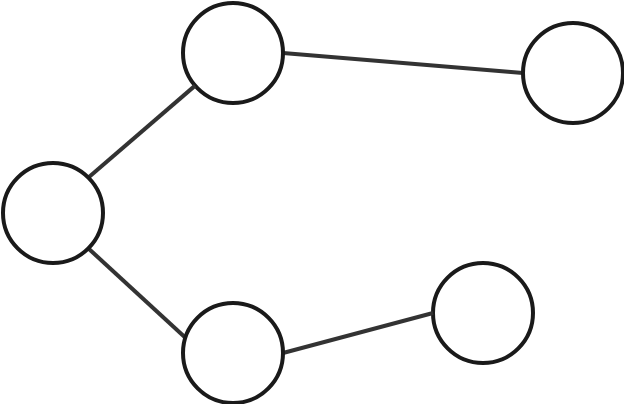
\includegraphics[width=0.5\textwidth]{img/G1.png}
		\caption{Graph G1.}
		\label{f1}
	\end{minipage}
	\hspace{0.1cm}
	\begin{minipage}[t]{0.5\linewidth} 
		\centering
		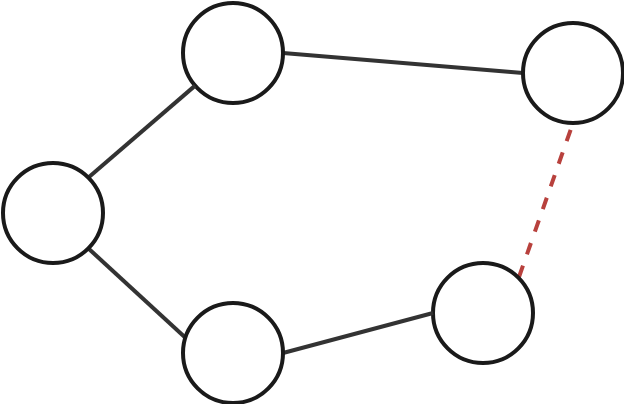
\includegraphics[width=0.5\textwidth]{img/G2.png}
		\caption{Graph G2.}
		\label{f2}
	\end{minipage}        
\end{figure} 

Here we can see that the two graphs are not the same, since G2 has an extra edge, but we can see that they are more or less similar. Considering only isomorphism as similarity we have 0 as result, instead we would like to define a new positive and simmetric similarity measure such that $K(G1,G2) = K(G2,G1) \geq 0$.




\section{Graph Kernel}
In section ~\ref{sec:graph_model} we have seen how data can be expressed in graphs and thanks to a technique called \textbf{kernel trick} we can use standard learning algorithm over them. \textbf{Graph kernels} are used for computing the similarity between pairs of graphs, based on common substructures they share and that can be computed in polynomial-time. Graph kernels are based on the idea of extrapolating patterns from the graphs and compare them, as follow it is presented an example of patterns that could be considered by a kernel.

 
 \begin{figure}[H]
 	\begin{minipage}[t]{0.5\linewidth}
 		\centering
 		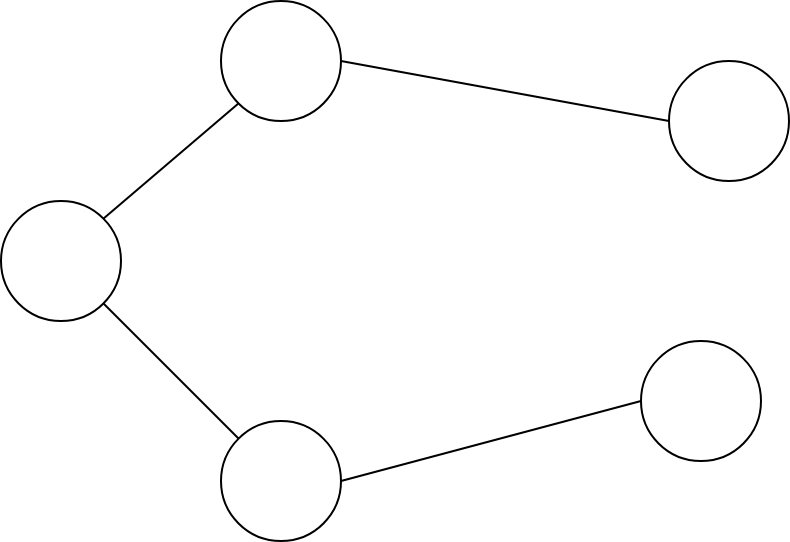
\includegraphics[width=0.5\textwidth]{img/graph_1.png}
 		\caption{Graph G1.}
 		\label{f1}
 	\end{minipage}
 	\hspace{0.1cm}
 	\begin{minipage}[t]{0.5\linewidth} 
 		\centering
 		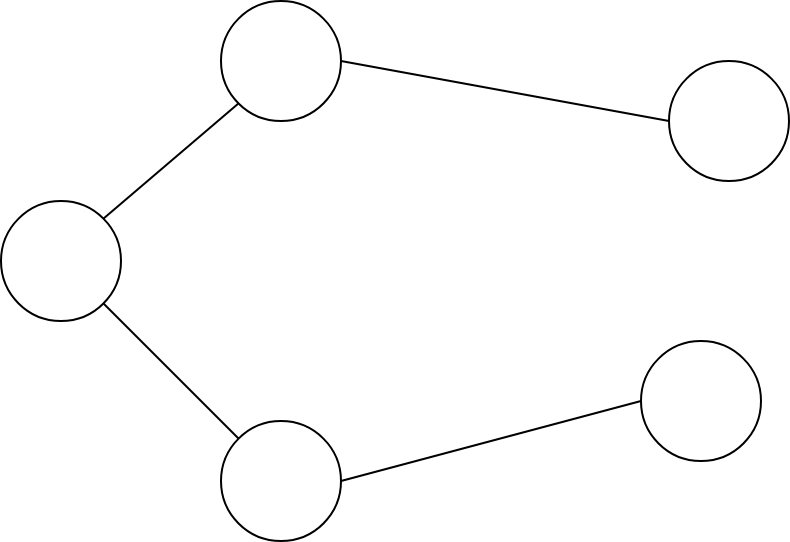
\includegraphics[width=0.5\textwidth]{img/graph_1.png}
 		\caption{Graph G2.}
 		\label{f2}
 	\end{minipage}        
 \end{figure} 

\image{img/k_patterns.png}{Kernel function between graph patterns}{0.6}


Since there isn't a unique and right way to describe similarity between graph, in literature are proposed different kernels that stand out by the way in which they localize patterns and compare them. An essential requirement for defining a kernel is that it must be a \textit{positive definite kernel}. The most used ones are so proposed:
\begin{itemize}
	\item \textbf{Shortest-path Kernel}
	\item \textbf{Random Walk Kernel}
	\item \textbf{Graphlet Kernel}
	\item \textbf{Weisfeiler-Lehman Kernel}
\end{itemize}
%During the following document we will discuss and analyze the results provided two different graph kernels, shortest-path and Weisfeiler-Lehman, that were used to study the given datasets.
Selecting the right kernel for a given application is a practical hurdle when applying kernel methods in practice. For this reason and to give a better idea of the various techniques, we will deal with two different graph kernels, shortest-path and Weisfeiler-Lehman, we will analyze their results on two datasets and their computational costs.

\subsection{Shortest-Path Kernel}
In literature we can find different kernels which base their similarity measure on the structure of the graph, like number of triangles, paths or walks. The idea of these approaches is to get and summarize the structure information of a given graph in something that can possibly represent the graph structure.
A very well know approach consists on enumerating all the paths of the two graphs and compare the similarity between the paths. The drawback of this solution is given by the time complexity required by the kernel, since until now the problem of enumerating all the paths in a graph is NP-hard and no polynomial time algorithm exists for it. \\
A similar approach consists not on computing all the paths, but only the shortest ones in the graph. Computing shortest paths in a graph, however, is a problem
solvable in polynomial time. Very well known algorithms such as Dijkstra, for shortest paths from one source node, or Floyd-Warshall, for all pairs of nodes, allow to determine shortest distances in polynomial time. From this idea of enumerating all the shortest paths and compare them between the two graphs comes the \textit{Shortest-Path Kernel}.

% $O(m+n*log n)$ and $O(n^3 )$ time, which is of .

\paragraph{Definition} Let $G = (V,E)$ be an undirected graph and let $S$ be its shortest-path graph,i.e., a graph defined over the same set of nodes $V$ where there exist an edge between two nodes if these are connected by a walk in $G$. The shortest-path kernel counts the numbers of common shortest-path in two graphs $G_1$ and $G_2$, that first are transformed into their corresponding shortest-path graphs $S_1 = (V_1, E_1)$ and $S_2 = (V_2, E_2)$ and then the kernel similarity is defined as:
$$K_{sp}(S_1,S_2) = \sum_{e_1\in E_1} k(e_1, e_2)$$
where $k$ is an arbitrary positive definite kernel that measures the similarity between the shortest paths corresponding to the edges $e_1$ and $e_2$.\\
\newpage

The shortest-path kernel algorithm is very simple and can be summarized in few steps:
\begin{itemize}
	\item Compute from the adjacency matrix of $G_1$ and $G_2$ the corresponding shortest paths ($S_1$ $S_2$), using a polynomial-time algorithm such as Floyd-Warshall.
	\item Define a similarity measure between paths and compare the set of paths previously generated. An example of measure could be the number of nodes in the shortest-path, or the number of nodes labels that are in common for each path.
\end{itemize} 



\subsection{Floyd-Warshall algorithm}
We have seen that the first step useful for computing the shortest path kernel between two graphs consists on computing all their shortest paths.  For this problem, a number of algorithms is known. Here it is provided a simple table that can summarize the time complexity required for each algorithm. 

\renewcommand{\arraystretch}{1.5}
\begin{table}[!htbp]
	\centering
	\begin{tabularx}{\linewidth}{|Y|l|l|l|}
		\cline{1-4}
		\centering{\textbf{G Structure $\backslash$ Algorithm}} & \thead{Dijkstra} & \thead{Bellman Ford} & \thead{Floyd Warshall}\\
		
		\cline{1-4}
		\centering \textit{Sparse graph} & $\quad\mathcal{O}(|V|^2\log|V|)\quad$ & $\quad\mathcal{O}(|V|^3)\quad$ & $\quad\mathcal{O}(|V|^3)\quad$ \\
		\cline{1-4}
		
		\cline{1-4}
		\centering \textit{Dense Graph} & $\quad\mathcal{O}(|V|^3\log|V|)\quad$& $\quad\mathcal{O}(|V|^4)\quad$ & $\quad\mathcal{O}(|V|^3)\quad$ \\
		\cline{1-4}
	\end{tabularx}%
		\caption{Shortest path algorithms complexities.}
\end{table}
\renewcommand{\arraystretch}{1}
We can see that the best case is given by Dijkstra's algorithm over sparse graphs, instead Floyd-Warshall algorithm maintains the same complexity in both of the two cases. In principle we can analyze the graphs dataset and decide what algorithm could give better performance, but in order to give good performance in general the Floyd-Warshall's algorithm could be an optimal compromise.
\begin{algorithm}
	\caption{Floyd-Warshall algorithm.}
	\begin{algorithmic}[1]
		\Procedure{\textbf{FW}}{$G$}\Comment{$G = (V,E)$}
		\State \textbf{Let} dist be a $|V| \times |V|$ array of minimum distances initialized to $\infty$.
		\For{\textbf{each} edge $(u,v)$}
			\State $dist[u,v] \leftarrow w(u,v)$ \Comment $w(u,v)$ weight of the edge $(u,v)$
		\EndFor
		
		
		\For{\textbf{each} vertex $v$}
			\State $dist[v,v] \leftarrow 0$ 
		\EndFor
		
		\For{ k \textbf{from} $1$ \textbf{to} $|V|$}

			
			\For{ i \textbf{from} $1$ \textbf{to} $|V|$}
			
				
				\For{ j \textbf{from} $1$ \textbf{to} $|V|$}
					\If{$\quad dist[i,j] > dist[i,k] + dist[k,j]$}
						\State $dist[i,j] = dist[i,k] + dist[k,j]$
					\EndIf
				\EndFor
			\EndFor
		\EndFor
		\EndProcedure
	\end{algorithmic}
\end{algorithm}


\begin{figure}[H]
	\begin{minipage}[t]{0.5\linewidth}
		\centering
		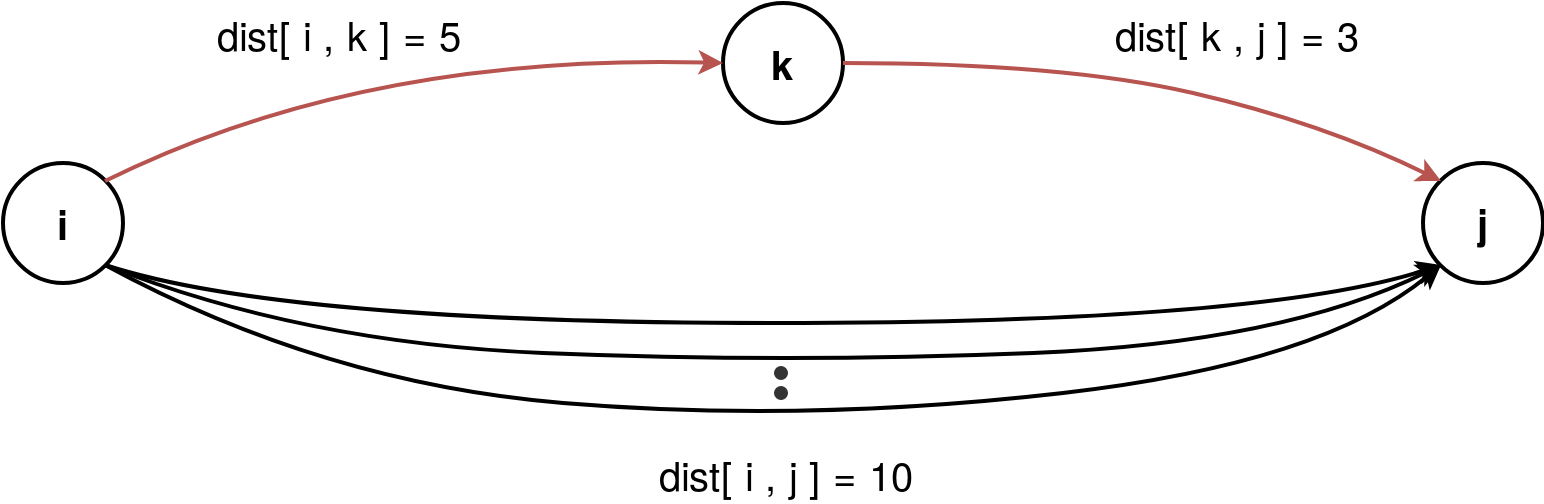
\includegraphics[width=0.9\textwidth]{img/FW_min.png}
		\caption{Floyd-Warshall path decision.}
		\label{f1}
	\end{minipage}
	\hspace{0.1cm}
	\begin{minipage}[t]{0.5\linewidth} 
		\centering
		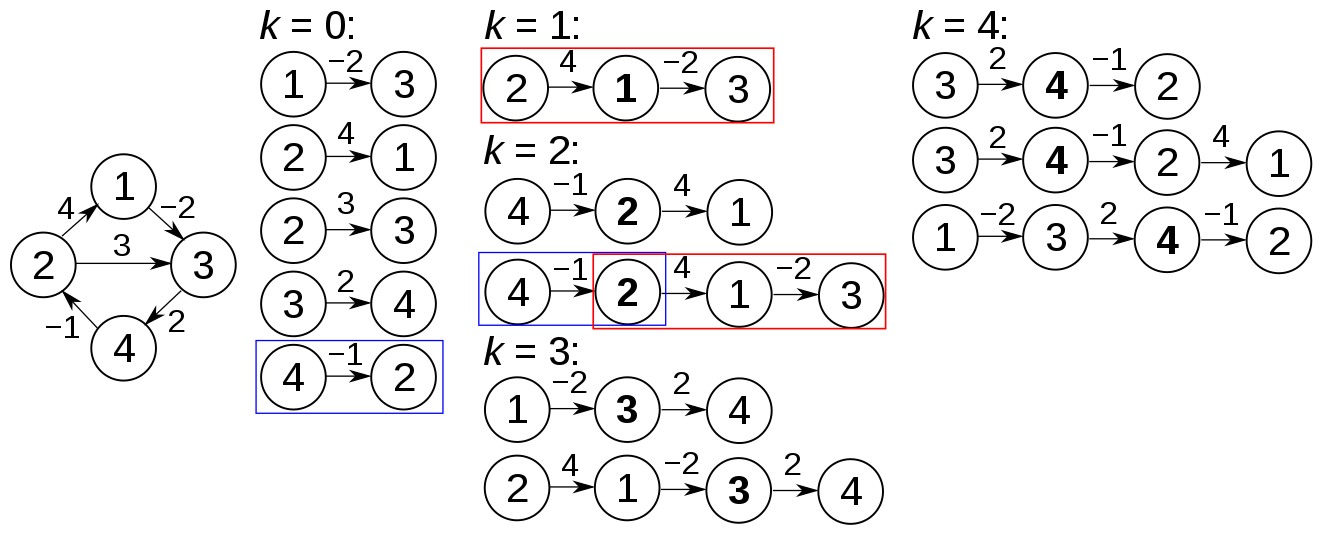
\includegraphics[width=0.9\textwidth]{img/FW_iteration.png}
		\caption{Floyd-Warshall iteration.}
		\label{f2}
	\end{minipage}        
\end{figure}
The major characteristic of the FW's algorithm is that at each iteration it discovers new paths, that pass from node k, and picks update the shortest paths considering the min between the current shortest path and the new one. So at the end of the procedure each node is connected to the others with a shortest path algorithm.\\

An important aspect of the Floyd-Warshall's algorithm is that it can be optimized if the adjacency matrix is symmetric. In our case the all the graphs are undirected graphs with weights $0$ or $1$, this means that we have a symmetric adjacency matrix and when we compute the path $dist[i,j]$ we can immediately conclude that $dist[j,i] = dist[i,j]$. The improved version so tries to address this property reducing the number of iterations required by the algorithm.
\begin{algorithm}
	\caption{Floyd-Warshall algorithm for symmetric graphs.}
	\begin{algorithmic}[1]
		\Procedure{\textbf{symmetric-FW}}{$G$}\Comment{$G = (V,E)$}
		\State \textbf{Let} dist be a $|V| \times |V|$ array of minimum distances initialized to $\infty$.
		\For{\textbf{each} edge $(u,v)$}
		\State $dist[u,v] \leftarrow w(u,v)$ \Comment $w(u,v)$ weight of the edge $(u,v)$
		\EndFor
		
		
		\For{\textbf{each} vertex $v$}
		\State $dist[v,v] \leftarrow 0$ 
		\EndFor
		
		\For{ k \textbf{from} $1$ \textbf{to} $|V|$}
		
		
		\For{ i \textbf{from} $1$ \textbf{to} $|V|$}
		
		
		\For{ j \textbf{from} $i$ \textbf{to} $|V|$}
		\State $dist[i,j]= dist[j,i] =$ \textbf{min}$(dist[i,j], dist[i,k] + dist[k,j])$
		\EndFor
		\EndFor
		\EndFor
		\EndProcedure
	\end{algorithmic}
\end{algorithm}

\subsection{Similarity between paths}
Once the shortest paths matrices are computed it is necessary to implement the similarity function $k$ between them:
$$ k:S_1\times S_2\rightarrow \mathbb{R} \qquad S_1 = |V_1| \times |V_1| \qquad S_2 = |V_2| \times |V_2|$$
In theory there is not a similarity measure between paths, but what can be done is to preserve structure/topological information about them in vectors and compute their similarity. In particular I decided to analyze two different approaches:

\paragraph{Steps Kernel} The step kernel $k_{steps}$ measures the similarity between two shortest paths graphs considering for each node the sum of all shortest paths always starting from the source node.
Here it is presented an example that considers two distinct graphs(2,6) taken from the PPI dataset and belonging into the acidovorax class.

\begin{figure}[H]
	\begin{minipage}[t]{0.5\linewidth}
		\centering
		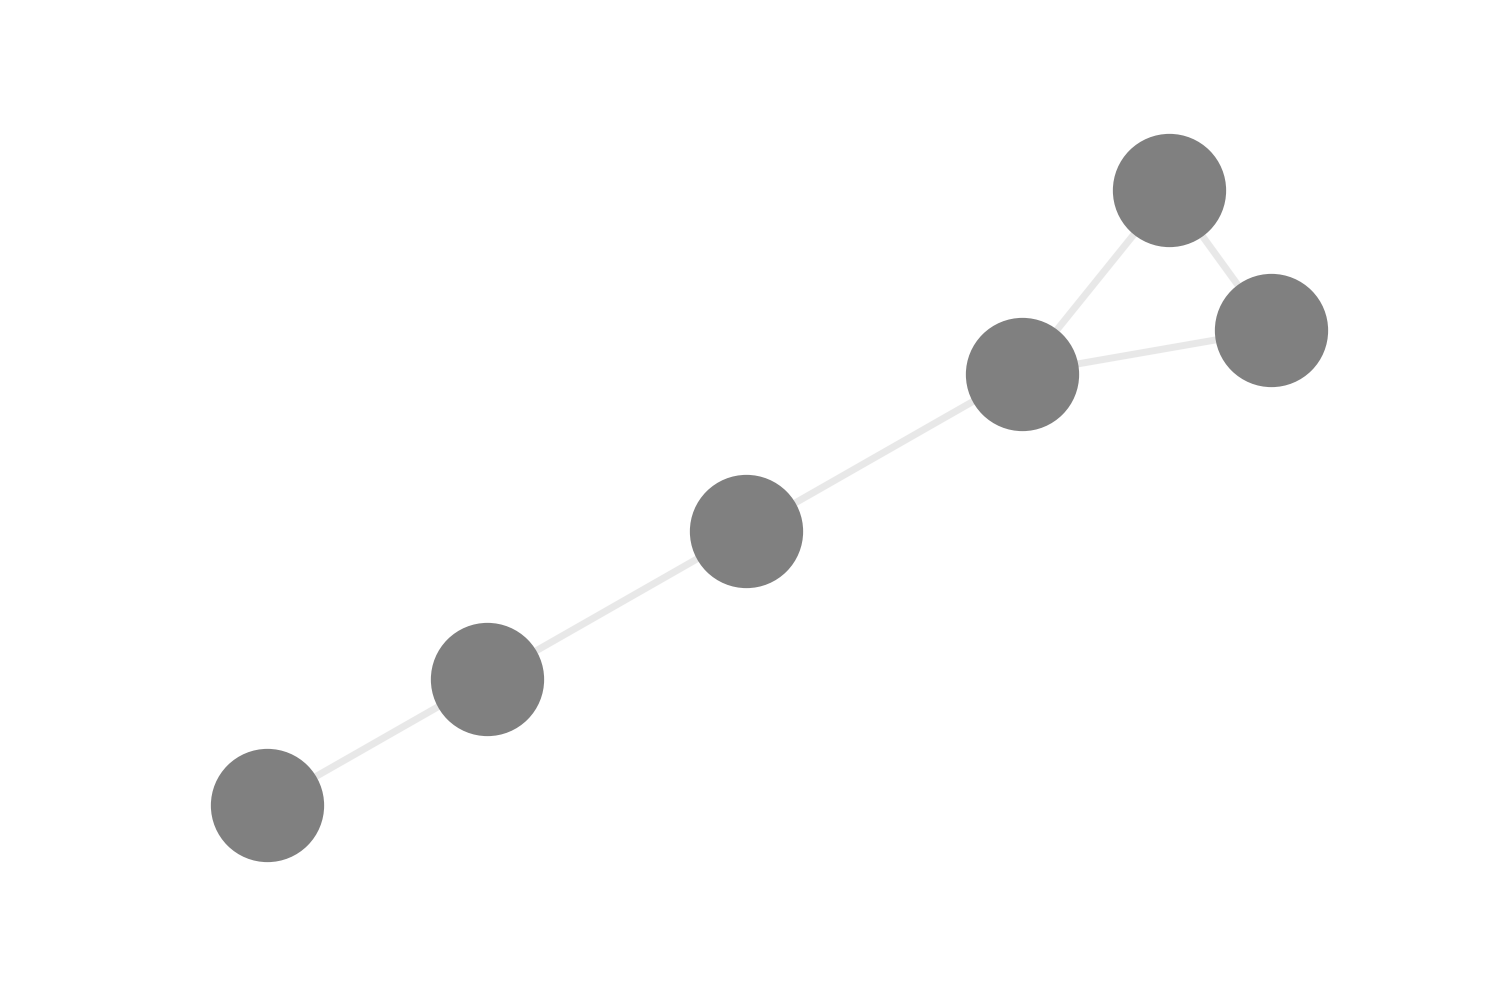
\includegraphics[width=0.7\textwidth]{img/acidovorax_graph_2am.png}
		\caption{$\text{Graph}_1$ adjacency matrix.}
		\label{f1}
	\end{minipage}
	\hspace{0.1cm}
	\begin{minipage}[t]{0.5\linewidth} 
		\centering
		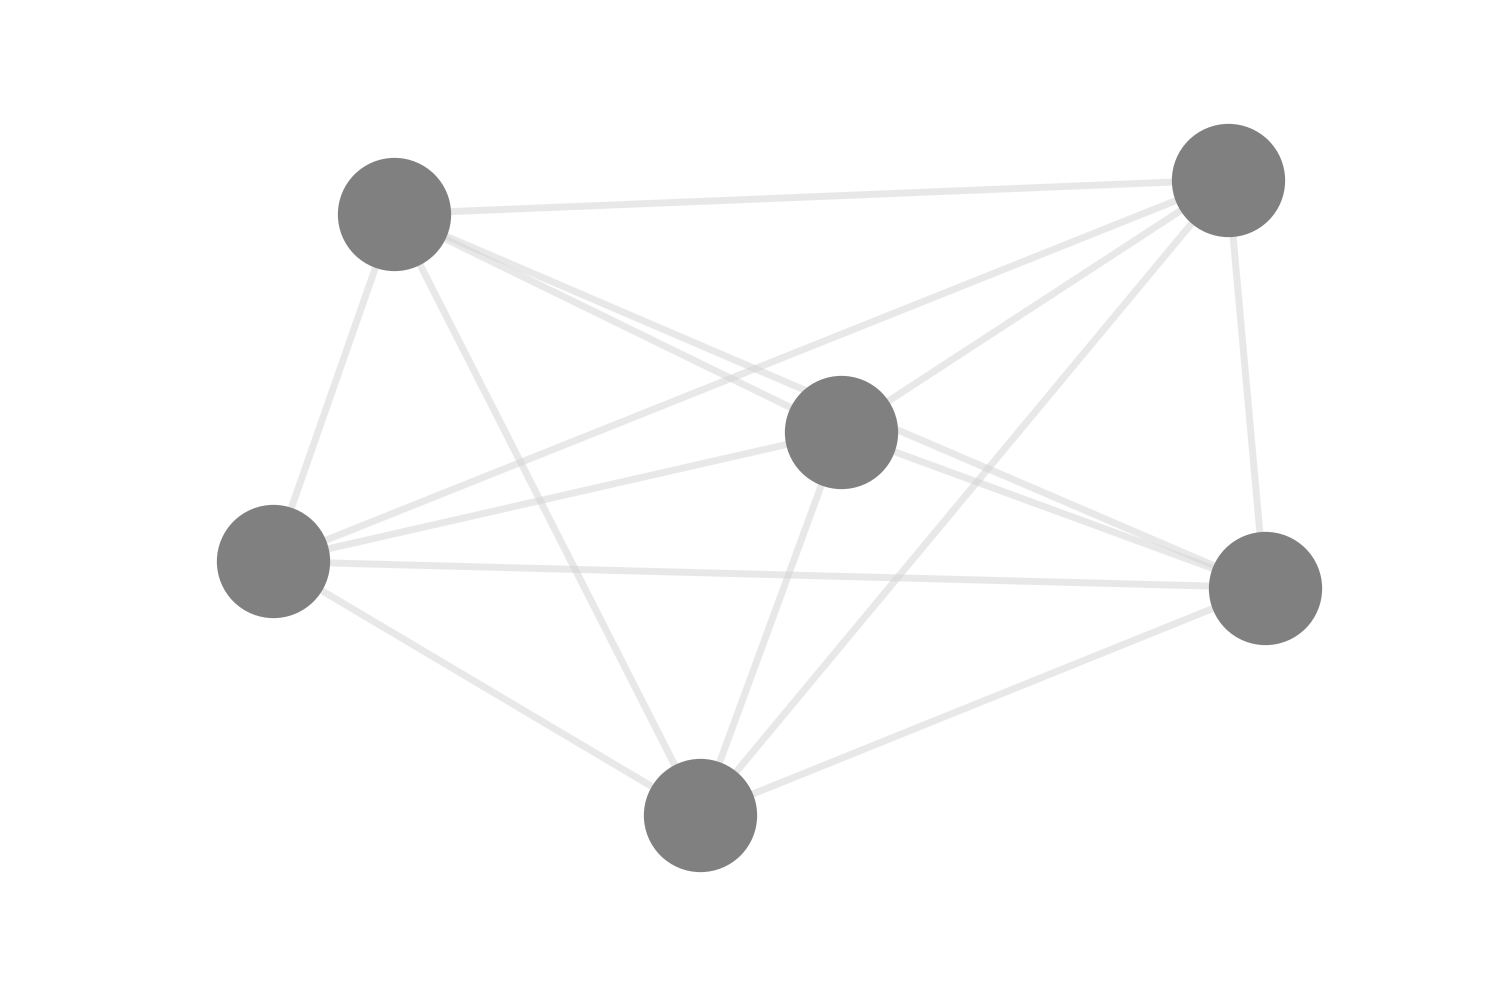
\includegraphics[width=0.7\textwidth]{img/acidovorax_graph_2sp.png}
		\caption{Shortest paths matrix.}
		\label{g1_w}
	\end{minipage}        
\end{figure}


\begin{figure}[H]
	\begin{minipage}[t]{0.5\linewidth}
		\centering
		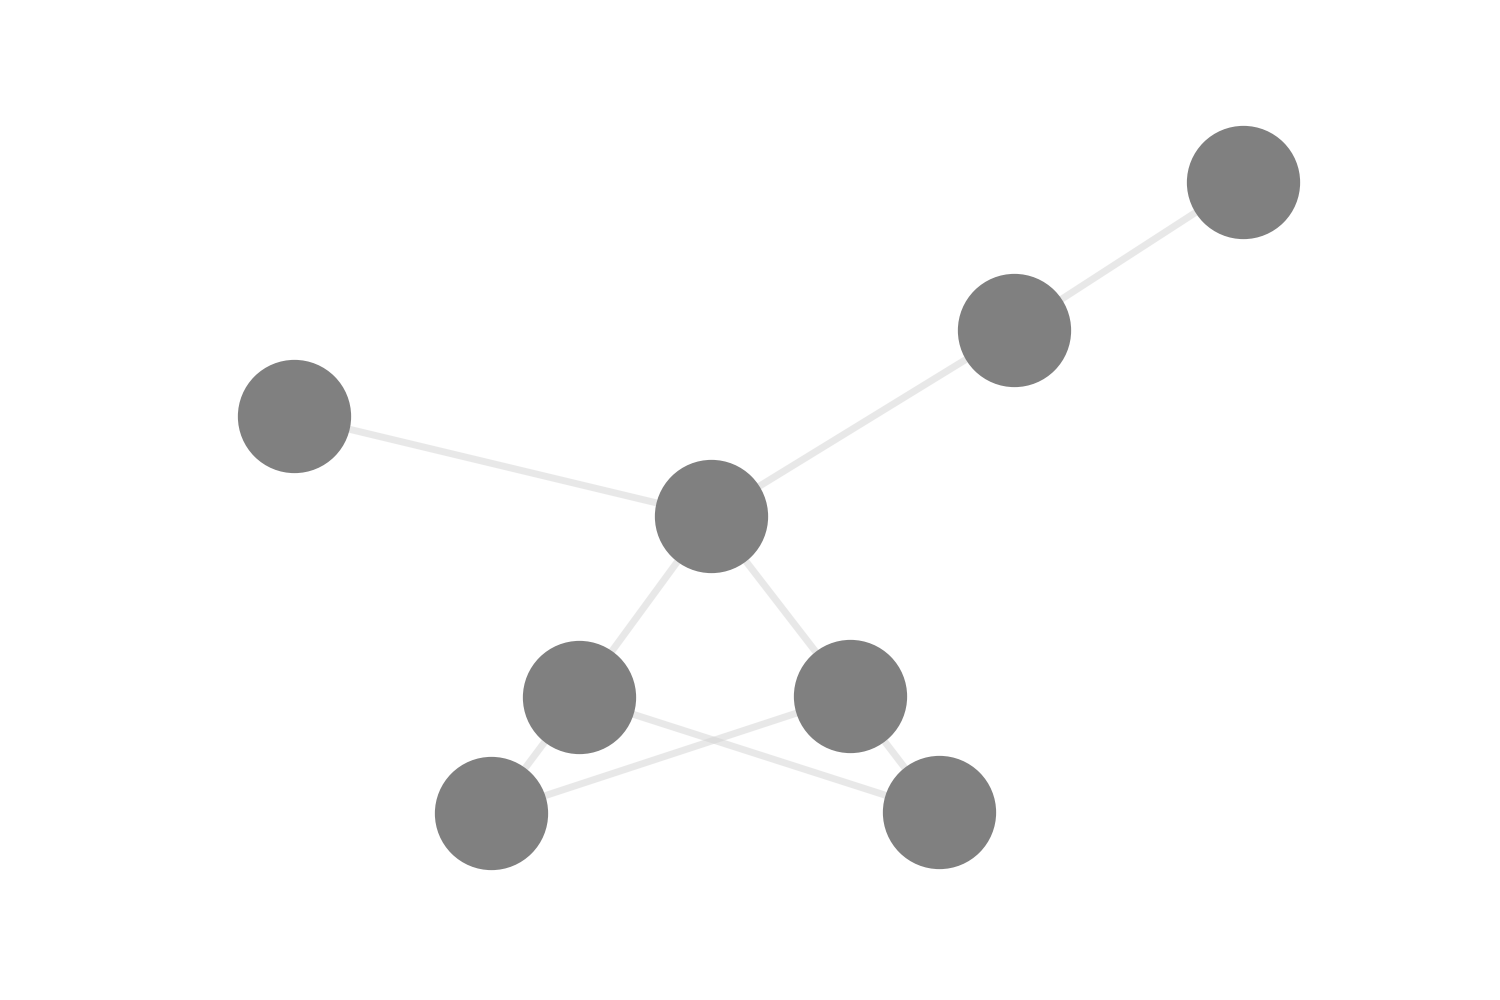
\includegraphics[width=0.7\textwidth]{img/acidovorax_graph_6am.png}
		\caption{$\text{Graph}_2$ adjacency matrix.}
		\label{f1}
	\end{minipage}
	\hspace{0.1cm}
	\begin{minipage}[t]{0.5\linewidth} 
		\centering
		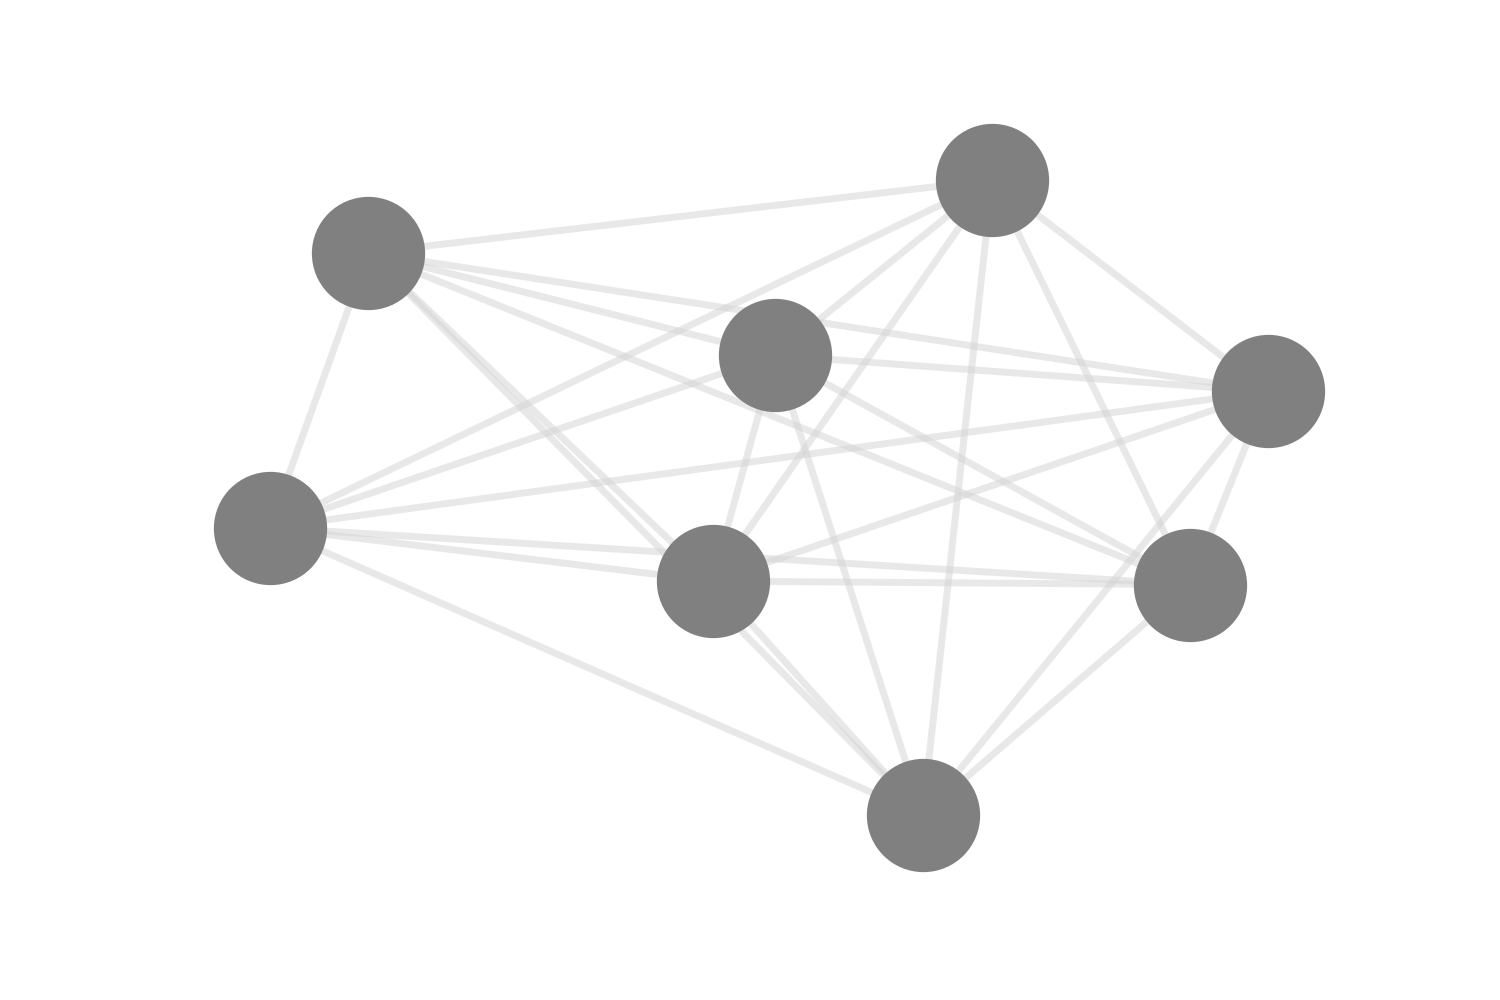
\includegraphics[width=0.7\textwidth]{img/acidovorax_graph_6sp.png}
		\caption{Shortest paths matrix.}
		\label{g2_w}
	\end{minipage}        
\end{figure}

Below are given the shortest paths matrices computed from $G_1$ and $G_2$, which are graphically represented on in Figure \ref{g1_w} and Figure \ref{g2_w}:
$$
SP_1 = \begin{bmatrix}
	0 & 1 & 1 & 3 & 4 & 2\\
	1 & 0 & 1 & 2 & 3 & 1\\
	1 & 1 & 0 & 3 & 4 & 2\\
	3 & 2 & 3 & 0 & 1 & 1\\
	4 & 3 & 4 & 1 & 0 & 2\\
	2 & 1 & 2 & 1 & 2 & 0
\end{bmatrix}
\qquad
SP_2 = \begin{bmatrix}
0 & 1 & 1 & 2 & 2 & 3 & 3 & 2\\
1 & 0 & 2 & 3 & 3 & 4 & 4 & 3\\
1 & 2 & 0 & 1 & 1 & 2 & 2 & 1\\
2 & 3 & 1 & 0 & 2 & 3 & 3 & 2\\
2 & 3 & 1 & 2 & 0 & 1 & 1 & 2\\
3 & 4 & 2 & 3 & 1 & 0 & 2 & 1\\
3 & 4 & 2 & 3 & 1 & 2 & 0 & 1\\
2 & 3 & 1 & 2 & 2 & 1 & 1 & 0
\end{bmatrix}
$$
Then the two shortest path matrices are reduced to the following vectors:
\image{img/k_w.png}{Vectorial reduction}{0.5}
Note that each position $i$ of these two vectors contains the sum of all the shortest paths that start from node $i$. Since graphs can have different number of nodes, the smaller one is padded with zeros (like SP1). Then, in order to compute their similarity, it is computed the dot product between them and normalization is performed so that the resulting similarity belongs to $[0,1]$. \\
Since we are using dot product between positive vectors we have the guarantee that the kernel is still positive definite.


\paragraph{Delta Kernel} The delta kernel $k_\delta$ measures the similarity between all the paths of two graphs considering the occurrences of each path's length. In other words, given a threshold $\delta$ we create a vector with dimension $\delta$ that represents the occurrences of paths with weights lower that $\delta$. The choice of $\delta$ can be useful to decide the level of approximation that we want to use and also to reduce the computational costs. For these experiences $\delta$ is chosen equal to the maximum path's weight between the two graphs.\\
Below is proposed an example of how this kernel works considering the two previous graphs:

$$\delta = max\Big\{ max\big\{ SP_1\big\}, max\big\{ SP_2\big\}\Big\} = 4$$

\image{img/delta_freq.png}{Delta vectors for $SP_1$ and $SP_2$}{0.3}
The $i-th$ cell of a frequency vectors contains the occurrences of path with weight equal to $i$. For example $G_1$ has exactly $6$ path with weight equal to $4$, which are: $$\Big\{  0 \rightarrow 4, 2 \rightarrow 4, 4 \rightarrow 0, 4 \rightarrow 2, 0 \rightarrow 4, 0 \rightarrow 4 \Big\}$$
Once the delta vectors are computed they are normalized and then the dot product between them is computed, so that at the end we have a similarity measure between $[0,1]$. Since we are using dot product between positive vectors we have the guarantee that the kernel is still positive definite.

\subsection{Weisfeiler-Lehman Kernel}
The Weisfeiler-Lehman (WL) kernel is based on the application of the WL test of isomorphism, more specifically its 1-dimensional variant, also known as \textit{naive vertex refinement}. Initially the WL method was considered as a way to solve the graph isomorphism problem in polynomial time, but then it was discovered that there are families of non-isomorphic pairs of graphs which cannot be solved correctly in polynomial time by this method.\\
Assume we are given two graphs $G$ and $G^\prime $ and we would like to test whether they are isomorphic, then the WL test is nothing else that an iterative procedure between the two graphs that compresses and propagates information in the nodes. In other words the key idea of the algorithm is to consider the node labels by the sorted set of node labels of neighbouring nodes, and compresses these augmented labels into new, short labels. These steps are then repeated until the node label sets of $G$ and $G^\prime$ differ, or the number of iterations reaches. \\
Respect to the shortest-path kernel the definition of a graph is a little bit different since now a graph $G$ is a triplet $G = (V, E, l)$, where now $l$ is a function returning the label of a node. 
In each iteration i of the Weisfeiler-Lehman algorithm  we get a new labeling $l_i(v)$ for all nodes $v$. Recall that this labeling is concordant in $G$ and $G^\prime$ , meaning that if nodes in $G$ and $G^\prime$ have identical multiset labels, and only in this case, they will get identical new labels.
In our datasets, nodes of graphs are not associated to a specific label, for that reason a first step of my algorithm was to define the function $l$ as the node degree function.\\

The developed instance of WL kernel is called \textbf{Weisfeiler-Lehman subtree kernel}.

\paragraph{Definition} Let $G$ and $G^\prime$ be graphs. Define $\Sigma_i \subset \Sigma$ as the set of letters that occur as node labels at least once in $G$ or $G^\prime$ at the end of the $i-th$ iteration of the Weisfeiler-Lehman algorithm. Let $\Sigma_0$ be the set of original node labels of $G$ and $G^\prime$. Assume all $\Sigma_i$ are pairwise disjoint. Without loss of generality, assume that every $\Sigma_i = \big\{\sigma_{i1},\dots,\sigma_{i|\Sigma_i|},\big\}$ is ordered. Define a map $c_i: \big\{G,G^\prime\big\} \times \Sigma_i \rightarrow \mathbb{N}$ such that $c_i(G,\sigma_{ij})$ is the number of occurrences of the latter $\sigma_{ij}$ in the graph $G$. \\
The Weisfeiler-Lehman subtree kernel on two graphs $G$ and $G^\prime$ with $h$ iterations is defined as:
$$ k^{(h)}_{\text{WLsubtree}}(G,G^\prime) = \langle \phi^{(h)}_{\text{WLsubtree}}(G), \phi^{(h)}_{\text{WLsubtree}}(G^\prime) \rangle$$
where
$$\phi^{(h)}_{\text{WLsubtree}}(G) = \big(c_0(G,\sigma_{01}),\dots,c_o(G,\sigma_{0|\Sigma_0|}), \dots, c_h(G,\sigma_{h1}), \dots, c_h(G,\sigma_{h|\Sigma_h|})  )\big)$$


$$\phi^{(h)}_{\text{WLsubtree}}(G^\prime) = \big(c_0(G^\prime,\sigma_{01}),\dots,c_o(G^\prime,\sigma_{0|\Sigma_0|}), \dots, c_h(G^\prime,\sigma_{h1}), \dots, c_h(G^\prime,\sigma_{h|\Sigma_h|})  )\big)$$
The key idea of the Weisfeiler-Lehman subtree kernel is to count the number of common original and compressed labels in two graphs. The greater is that number the more similar are the two graphs.\\
The developed algorithm is composed by 4 essential steps:
\begin{enumerate}
	\item \textbf{Multiset-label determination}, for each of the two graph a label is determined. Each node label is composed by its original label and all the labels of the adjacent nodes, creating a multiset of labels.
	\item \textbf{Sorting}, for each node the labels inside the multiset is sorted.
	\item \textbf{Label compression}, maps each string of labels to a compressed label.
	\item \textbf{Relabeling}, assigns to each node its compressed label.
\end{enumerate}

\begin{algorithm}
	\caption{One iteration of the WL subtree kernel computation on N graphs.}
	\begin{algorithmic}[1]

		\State Multiset-label determination
		\begin{itemize}
			\item Assign a multiset-label $M_i(v)$ to each node $v$ in $G$ which consists of the multiset $\big\{l_{i-1}(u)|u\in \mathcal{N}(v)\big\}$\Comment$\mathcal{N}(v)$ list of neighbors of $v$	
		\end{itemize}
	
		\State Sorting each multiset
		\begin{itemize}
			\item Sort elements in $M_i(v)$ in ascending order and concatenate them into a string $s_i(v)$.
			\item Add $l_{i-1}(v)$ as a prefix to $s_i(v)$
		\end{itemize} 
		
		\State Label compression
		\begin{itemize}
			
			\item Map each string $s_i(v)$ to a compressed label using a hash function $f:\Sigma^* \rightarrow \Sigma$ such that $f(s_i(v)) = f(s_i(w))$ if and only if $s_i(v)$ = $s_i(w)$. 
		\end{itemize}
		\State Relabeling
		\begin{itemize}
			\item Set $l_i(v):= f(s_i(v))$ for all nodes in $G$.
		\end{itemize}		

	\end{algorithmic}
\end{algorithm}
\image{img/WLalgorithm.png}{WL subtree kernel algorithm steps}{0.65}
\image{img/WLresult.png}{End of the 1st iteration
	Feature vector representations of $G$ and $G^\prime$}{0.55}

In theory is also proved that for $N$ graphs, the Weisfeiler-Lehman subtree kernel with $h$ iterations on all pairs of these graphs can be computed in $O(Nhm + N^2hn)$. This complexity here comes from the fact that computing $\phi^{(h)}_{\text{WLsubtree}}$ has a complexity equal to $O(Nhm)$, assuming that $m > n$. The number of iteration $h$ defines how much the information between nodes are propagated, so the greater it is the more information about the graph we have. In case $h$ is limited by an upper bound beyond which no extra information is extracted and the algorithm reaches a stationary point.

\section{Manifold Learning}
Real-world data, such as speech signals, images, ecological data or data on health status, usually has a high dimensionality, which means that they are composed by a large set of features. Intuitively we could think that the greater is the level of information that we have the best are the results, but this statement is not always good. When analyzing huge sets of numerical data, problems often occur when the raw data are high-dimensional. This problem was firstly discussed by  Richard E. Bellman who gives to it the name of \textbf{curse of dimensionality}, which refers to the problem of finding structure in data embedded in a highly dimensional space. In other words, when the dimensionality of data increases the volume of the space increases too and available data become sparse, and the result of this situation is that all data points appear to be sparse and dissimilar in many ways. Many algorithms, like KNN in which we need to find the nearest neighbor, tend to perform very well with low-dimensional data, but their complexity increase when we increase dimensionality of data. Note also that for humans it is not possible to perceive data in a very \textbf{high-dimensional space}, so reducing the dimensionality of data to two or three and visualizing embedded data has become increasingly useful for multivariate analysis.\\
In literature we can find different dimensionality reduction techniques widely used for the analyzing and visualize complex sets of data. These techniques can be classified in linear or non-linear ones.
One of the first and most common method of dimension reduction is \textbf{principle component analysis} (PCA), which is basically a linear technique based on preserving the maximum explained variability. PCA finds the directions along which the data has maximum variance in addition to the relative importance of these directions. The main assumption of PCA is that the principle components are a linear combination of the original features. If this is not true, PCA could not provide accurate results. \\
However, nonlinear structures are rather common in real data and it is necessary to introduce more sophisticated models like \textbf{manifold learning}. Manifold learning algorithms are based on the idea that the dimensionality of many data sets is only artificially high. Although the data points may consist of thousands of features, they may be described as a function of only a few underlying parameters. That is, the data points are actually samples from a low-dimensional manifold that is embedded in a high-dimensional space. Manifold learning algorithms attempt to extract a low-dimensional representation that represent as better as possible high-dimensional data.\\

The most famous manifold learning technique are:
\begin{itemize}
	\item \textbf{Isomap}
	\item \textbf{Diffusion Map}
	\item \textbf{Laplacian Eigenmaps}
	\item \textbf{Local Linear Embedding}
\end{itemize}
The goal of this assignment is to use different manifold learning techniques to the distance matrix in order to increase if possible the class separation. The distance matrix $D = (d_{ij})$ is computed starting from the kernel matrix $K = (k_{ij})$ obtained from the previous explained graph kernels over a set of $n$ graphs. In particular $D$ is computed as follow:
$$d_{ij} = \sqrt{k_{ii} + k_{jj} - 2k_{ij}}$$
Then a linear SVM is used for learning data and class separation. The rest of the document will provide some theoretical knowledges about two manifold learning techniques, isomap and local linear embedding, and performance over the two dataset.

\subsection{Isomap}
Isomap, short for Isometric Feature Mapping, has been one of the first algorithms introduced for manifold learning and has gained significant popularity due to its conceptual simplicity and efficient implementation. Isomap can be seen as a generalization of \textbf{Multidimensional Scaling} (MDS) where the distance metric is the \textbf{geodesic distances}. Geodesics are lines of shortest length between points on a manifold, which act like straight lines on a plane. \\
The key idea of geodesic distance is that it preserves global isometries. Multi-dimensional data space is often curved rather than Euclidean and the simplest example is given by data points placed along a sphere, like Figure \ref{geo1}. 


\begin{figure}[H]
	\begin{minipage}[t]{0.5\linewidth}
		\centering
		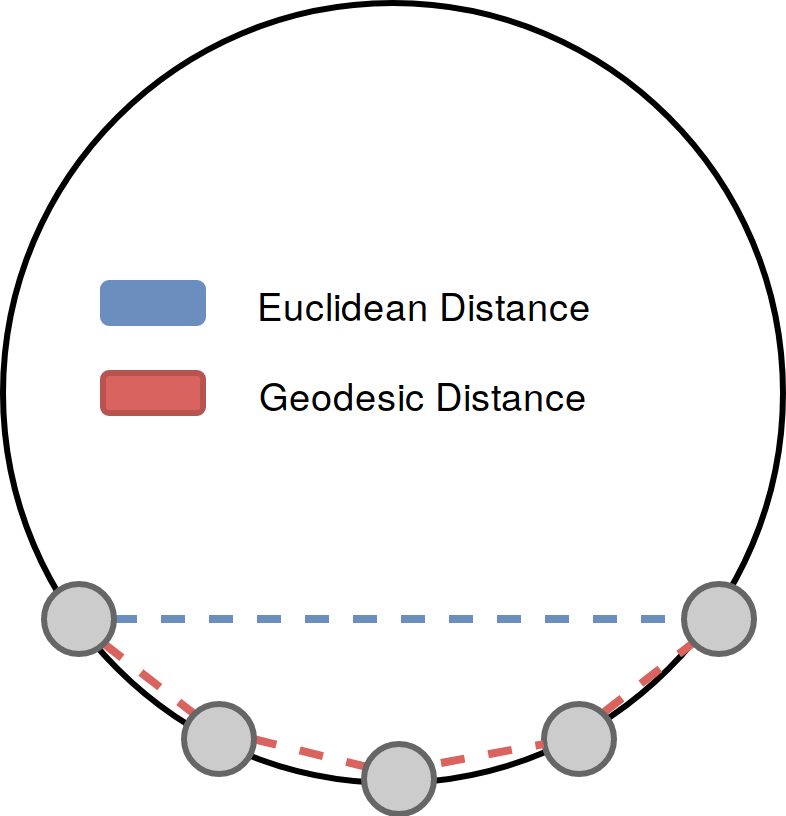
\includegraphics[width=0.65\textwidth]{img/geodesic.png}
		\caption{Distances on a sphere manifold.}
		\label{geo1}
	\end{minipage}
	\hspace{0.1cm}
	\begin{minipage}[t]{0.5\linewidth} 
		\centering
		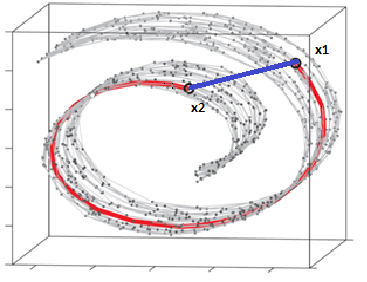
\includegraphics[width=0.8\textwidth]{img/geo2.png}
		\caption{Distances on a real data manifold.}
		\label{geo2}
	\end{minipage}        
\end{figure}
From Figure \ref{geo1} we can see that distances among the points are best measured by the geodesic distance since it preserves distances along the surface of the sphere rather than the direct measure through the sphere. A simple approximation of the geodesic distances assumes that the distance between close points can be well approximated by the Eucledian distance and the distance between points which are farther is estimated considering the length of the shortest path between them. In other words the curvature of the space can be approximated through a network, then:
\begin{itemize}
	\item if nodes $i$ and $j$ are close then the effect of curvature is minimal and the Eucledian distance is a good estimator for the geodesic distance.
	\item if nodes $i$ and $j$ are farther then we can have a strong curvature along the manifold so the geodesic distance is estimated as the length of the minimal path between $i$ and $j$ on a neighborhood graph.
\end{itemize}
Given a collection of $n$ objects on which a distance function between objects $\delta_{i,j}$ is defined, we compute the dissimilarity matrix $\Delta$, which is so defined: 

$$\Delta = 
\begin{pmatrix}
	\delta_{1,1} & \delta_{1,2} & \cdots & \delta_{1,n} \\
	\delta_{2,1} & \delta_{2,2} & \cdots & \delta_{2,n} \\
	\vdots & \vdots & & \vdots \\
	\delta_{n,1} & \delta_{n,2} & \cdots & \delta_{n,n}
\end{pmatrix}
$$
where  $\delta_{i,j} =$ distance between $i$-th and $j$-th objects.\\
Then the goal of MDS is to find $n$ vectors $x_1,\dots,x_n \in \mathbb{R}^N$ starting from $\Delta$, such that:
$$ ||x_i - x_j|| \sim \delta_{i,j} \qquad \forall i,j \in 1,\dots,n$$
The vectors $x_1,\dots,x_n$ represents the embedding from the objects into a new space $\mathbb{R}^N$ in which distances are preserved.\\
Respect to the MDS procedure Isomap uses the geodesic distance as distance function, with the goal of preserving global isometries and distances between points.\\

Isomap algorithm can be summarized in the following steps:
\begin{itemize}
	\item Step 1: Given data set $x_i \in R^D$ , form the weighted \textbf{k}-nearest
	neighbor graph $G$. That is put edge between vertices $x_i$ and $x_j$ if $x_j$
	is one of the \textbf{k} nearest neighbors of $x_i$ or vice versa in the Euclidean
	distance. It assigns each edge $(x_i, x_j)$ weight $kx_i - x_jk$.
	\item Step 2: Compute the shortest path distances between all pair of vertices
	$x_i$ and $x_j$ store it in $S_{ij}$. This can be done using Floyd-Warshall's or by Dijkstra's algorithm and storing the square of the shortest path into distance matrix $D_{ij} = S_{ij}$.
	\item Step 3: Apply MDS algorithm with dissimilarity matrix $D$ from previous step.
\end{itemize}

Isomap seems to not perform well when manifold is not well sampled and contains holes, for instance when we have disjoint parts. From a computation point of view neighborhood graph creation is tricky, expensive and slightly wrong parameters can produce bad results since the use of geodesic distances makes Isomap strongly dependent to the topology of the neighborhood graph.

\subsection{Local Linear Embedding}
Local Linear Embedding (LLE) is another strategy that can be adopted for nonlinear dimensionality reduction problems. The idea of this manifold technique is to reconstruct each data point on the manifold from its neighbors, provided that there is a sufficient amount of data. The expected behavior of a manifold is that each data point and its neighbors to lie on or close to a locally linear patch of the manifold. In the simplest formulation of LLE identifies $K$ nearest neighbors per data point, using metrics like Euclidean distance, and then the following cost function is evaluated:
$$ \epsilon(W) = \sum_i |{X_i - \sum_j {W_{ij}X_j}|}^2 $$
where the weights $W_{ij}$ indicate the contribution of each data point to the reconstruction. There is a unique constraint on the weights:
$$ \sum_j {W_{ij}} = 1 $$
The proposed cost function adds up the squared distances between all the data points and their reconstructions, so the lower it is the better is the approximation ability of the $K$ points. The goal of LLE is to solve a constraint problem that minimize the cost function $\epsilon(W)$.
The desirable behavior is that the local geometry in the original data space is maintained equally valid for local patches on the manifold. In particular, the same weights $W_{ij}$ that reconstruct the $i$-th data point in dimensions $D$ should also reconstruct its embedded manifold coordinates in $d$-dimensions, with $d \ll D$.\\

An important theoretical result is that the optimal weights $W$ are invariant to some transformation like rotation, re-scaling and translations to all the data points in the manifold. \\

In summary the LLE algorithm can be shortly summarized in the following steps:
\begin{itemize}
	\item Compute the neighbors of each data point $x_i$
	\item Compute the weights $W_{ij}$ that best reconstruct each data point $x_i$ from its neighbors, minimizing the cost $\epsilon(W)$.
	\item Each high dimensional observation $x_i$ is mapped to a low dimensional vector $y_i$ representing global internal coordinates on the manifold. This is done by choosing $d$ dimensional coordinates $y_i$ to minimize the embedding cost function:
	
	$$ \phi(y) = \sum_i |y_i - \sum_j {W_{ij}y_j}|^2 $$
	which indicates the locally linear reconstruction error fixing the weights $W_{ij}$. The focus of the optimization problem is to find the coordinated $y_i$ that minimize the cost function $\phi(y)$.
\end{itemize}

\begin{figure}[H]
	\begin{minipage}[t]{0.5\linewidth}
		\centering
		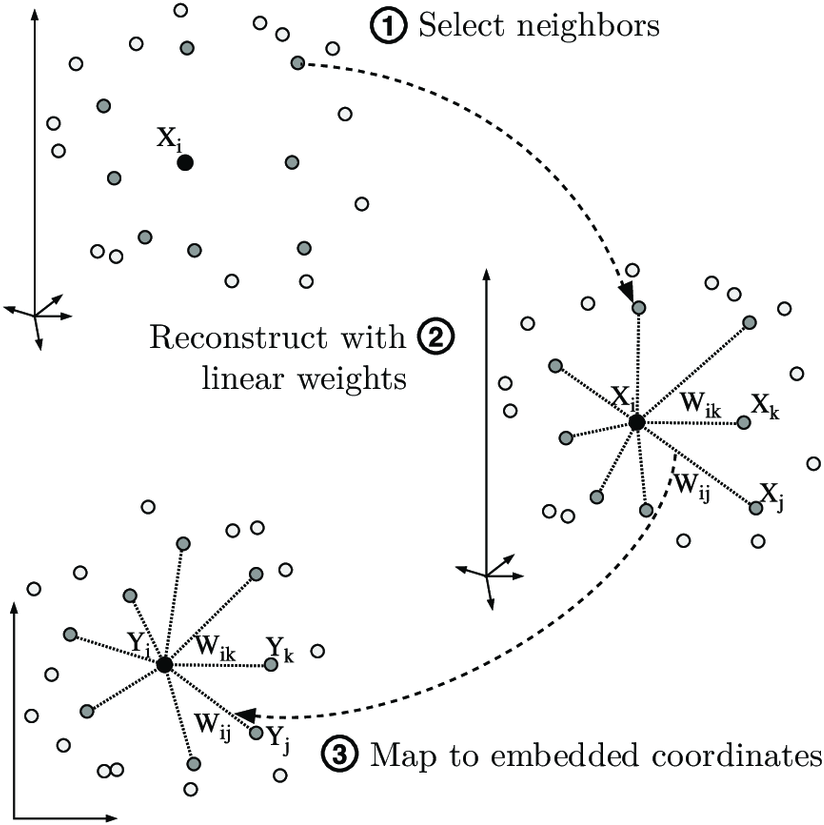
\includegraphics[width=0.6\textwidth]{img/LLEAlgorithm.png}
		\caption{Distances on a sphere manifold.}
	\end{minipage}
	\hspace{0.1cm}
	\begin{minipage}[t]{0.5\linewidth} 
		\centering
		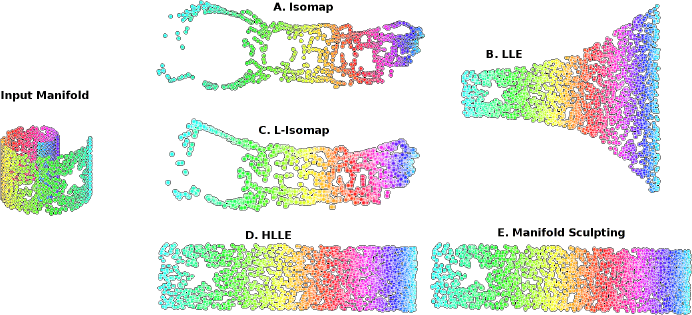
\includegraphics[width=0.9\textwidth]{img/comparison.png}
		\caption{Distances on a real data manifold.}
		\label{comparison}
	\end{minipage}        
\end{figure}

As we can see from Figure \ref{comparison} the presence of an hole in the manifold produce not well results, instead LLE seems to be more robust for the manifold embedding.

\section{Experimental Results and Comparison}
In this section it is presented and analyzed the different results provided by the combination of the various kernels, parameters and manifold learning techniques on the two datasets of graphs (PPI and Shock). First of all are proposed the results obtained without the application of any manifold learning technique, so the resulting scores will be retrieved from an SVM over the graph kernel distances. Secondly are proposed the results with the two techniques of manifold learning (Isomap, LLE) will be provided. At the end of the section it is analyzed the general behavior of the applied techniques and possible patterns or dependencies.

\subsection{PPI dataset}
First are proposed the results obtained from the PPI dataset.

\renewcommand{\arraystretch}{1.5}
\begin{table}[H]
	\centering
	\begin{tabularx}{\linewidth}{|Y|l|l|l|l|}
		\cline{1-5}
		\centering{\textbf{Kernel}} & \thead{min score} & \thead{avg score} & \thead{max score} & \thead{stand dev}\\
		
		\cline{1-5}
		\centering \textit{SP kernel - step} & $0.5$ & $0.692$ & $0.877$ & $0.133$\\
		\cline{1-5}
		
		\cline{1-5}
		\centering \textit{SP kernel - delta} & $0.625$ & $0.779$ & $0.888$ & $0.098 $\\
		\cline{1-5}
		
		\cline{1-5}
		\centering \textit{$WL_1$ Kernel} &$0.666$ & $\mathbf{0.8138^*}$ & $1$ & $0.132$\\
		\cline{1-5}
		\centering \textit{$WL_2$ Kernel} &$0.555$ & $0.775$ & $1$ & $0.113$\\
		\cline{1-5}
		
		\centering \textit{$WL_3$ Kernel} &$0.5$ & $0.752$ & $0.888$ & $0.189$\\
		\cline{1-5}
	\end{tabularx}
		\caption{PPI classification accuracy and standard error without manifold learning.}
		\label{table:svmPPI}
\end{table}
\renewcommand{\arraystretch}{1}

\renewcommand{\arraystretch}{1.5}
\begin{table}[H]
	\centering
\begin{tabular}{cc|c|c|c|c|l}
	\cline{3-6}
	& & \multicolumn{2}{ c| }{\textbf{Isomap}}& \multicolumn{2}{ c| }{\textbf{LLE}} \\ 
	\cline{1-6}
		\multicolumn{1}{ |c|  }{\#\textit{neighbors}}& \#\textit{dimensions}&\textit{avg} &\textit{std} & \textit{avg} & \textit{std} \\ 
	\cline{1-6}
	
	\multicolumn{1}{|c|}{1}& $6$ & $0.511$ & $0.042$ & $0.567$ & $0.069$\\
	\cline{1-6}
	\multicolumn{1}{|c|}{1 }& $17$ & $0.547$ & $0.128$ & $0.719$ & $0.062$\\
	\cline{1-6}
	\multicolumn{1}{|c|}{1 }& $18$ & $0.524$ & $0.116$ & $\mathbf{0.779^*}$ & $\mathbf{0.108^*}$\\
	\cline{1-6}
	\multicolumn{1}{|c|}{4 }& $11$ & $0.664$ & $0.181$ & $0.607$ & $0.109$\\
	\cline{1-6}
	\multicolumn{1}{|c|}{4 }& $18$ & $\mathbf{0.781^*}$ & $\mathbf{0.128^*}$ & $0.735$ & $0.108$\\
	\cline{1-6}
	\multicolumn{1}{|c|}{4 }& $24$ & $0.699$ & $0.181$ & $0.732$ & $0.113$\\
	\cline{1-6}
	\multicolumn{1}{|c|}{10}& $23$ & $0.662$ & $0.151$ & $0.757$ & $0.159$\\
	\cline{1-6}
	\multicolumn{1}{|c|}{16}& $17$ & $0.733$ & $0.184$ & $0.71$ & $0.123$\\
	\cline{1-6}
	\multicolumn{1}{|c|}{19}& $4$ & $0.701$ & $0.13$ & $0.556$ & $0.096$\\
	\cline{1-6}
	\multicolumn{1}{|c|}{19}& $16$ & $0.721$ & $0.149$ & $0.708$ & $0.083$\\
	\cline{1-6}
\end{tabular}
		\caption{PPI classification accuracy and std with m.l. and shortest path kernel.}
		\label{table:svmPPISPML}
\end{table}
\renewcommand{\arraystretch}{1}


%\image{img/Isomap_plots.png}{Isomap performance}{1}
%\image{img/LLE_plots.png}{LLE performance}{1}


\begin{figure}[H]
	\begin{minipage}[t]{0.5\linewidth}
		\centering
		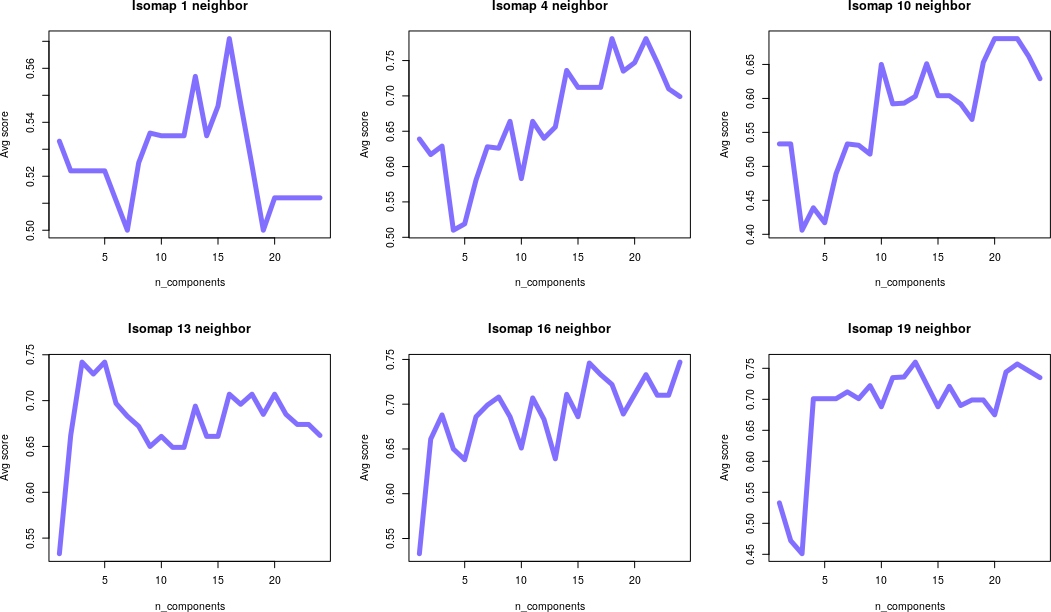
\includegraphics[width=1\textwidth]{img/Isomap_plots.png}
		\caption{Isomap performance.}
		\label{f1}
	\end{minipage}
	\hspace{0.1cm}
	\begin{minipage}[t]{0.5\linewidth} 
		\centering
		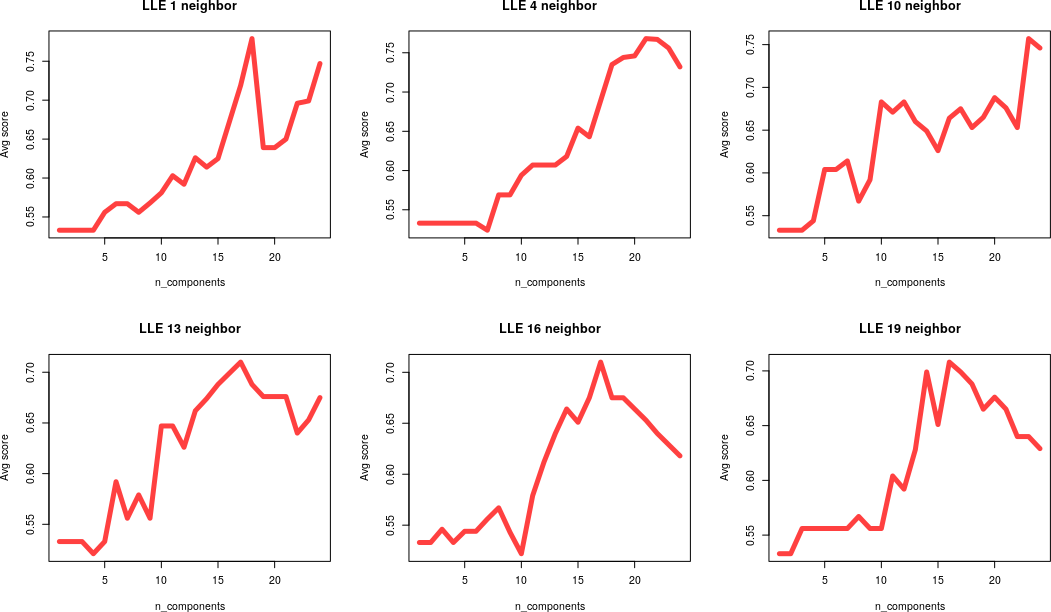
\includegraphics[width=1\textwidth]{img/LLE_plots.png}
		\caption{LLE performance.}
		\label{g1_w}
	\end{minipage}        
\end{figure}




\renewcommand{\arraystretch}{1.5}
\begin{table}[H]
	\centering
	\begin{tabular}{cc|c|c|c|c|l}
		\cline{3-6}
		& & \multicolumn{2}{ c| }{\textbf{Isomap}}& \multicolumn{2}{ c| }{\textbf{LLE}} \\ 
		\cline{1-6}
		\multicolumn{1}{ |c|  }{\#\textit{neighbors}}& \#\textit{dimensions}&\textit{avg} &\textit{std} & \textit{avg} & \textit{std} \\ 
		\cline{1-6}
			\multicolumn{1}{|c|}{1}& $17$ & $0.476$ & $0.108$ & $0.593$ & $0.077$\\
			\cline{1-6}
			\multicolumn{1}{|c|}{4}& $11$ & $0.724$ & $0.134$ & $0.636$ & $0.093$\\
			\cline{1-6}
			\multicolumn{1}{|c|}{4}& $18$ & $0.7$ & $0.145$ & $0.672$ & $0.112$\\
			\cline{1-6}
			\multicolumn{1}{|c|}{4}& $24$ & $0.606$ & $0.177$ & $0.721$ & $0.096$\\
			\cline{1-6}
			\multicolumn{1}{|c|}{10}& $8$ & $0.708$ & $0.127$ & $0.719$ & $0.08$\\
			\cline{1-6}
			\multicolumn{1}{|c|}{10}& $17$ & $\mathbf{0.815^*}$ & $\mathbf{0.112^*}$ & $0.718$ & $0.102$\\
			\cline{1-6}
			\multicolumn{1}{|c|}{16}& $9$ & $0.749$ & $0.162$ & $0.662$ & $0.108$\\
			\cline{1-6}
			\multicolumn{1}{|c|}{16}& $17$ & $0.719$ & $0.112$ & $\mathbf{0.79^*}$ & $\mathbf{0.069^*}$\\
			\cline{1-6}
			\multicolumn{1}{|c|}{19}& $4$ & $0.674$ & $0.099$ & $0.661$ & $0.071$\\
			\cline{1-6}
			\multicolumn{1}{|c|}{19}& $16$ & $0.676$ & $0.152$ & $0.71$ & $0.088$\\
			\cline{1-6}
\end{tabular}
		\caption{PPI classification accuracy and std with m.l. and Weisfeiler-Lehman kernel.}
		\label{table:svmPPIWLML}
\end{table}

\begin{figure}[H]
	\begin{minipage}[t]{0.5\linewidth}
		\centering
		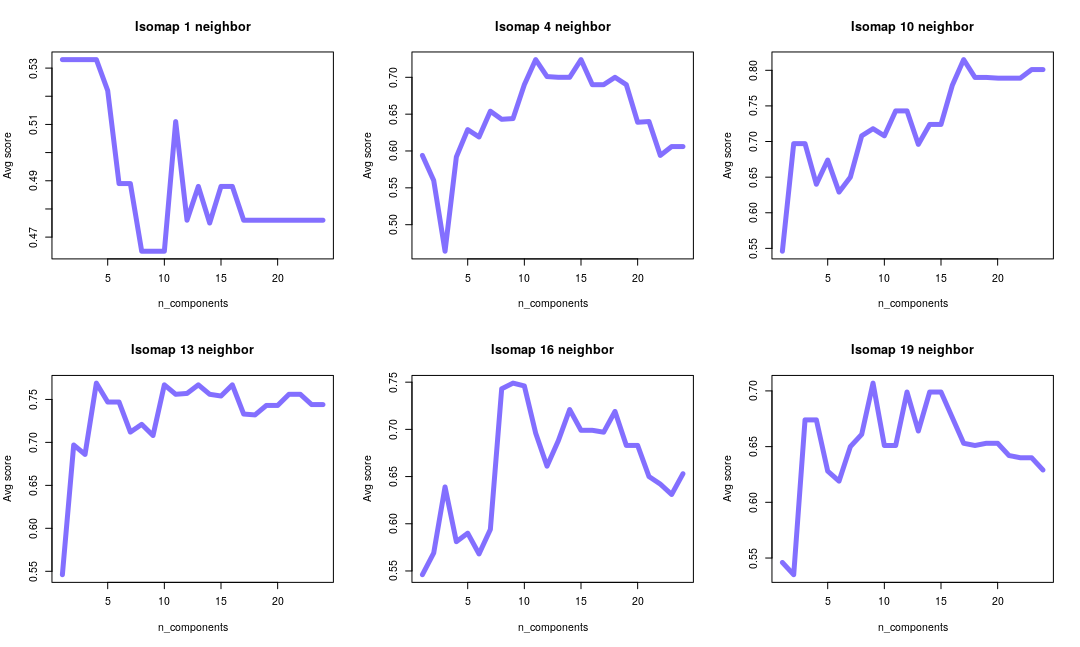
\includegraphics[width=1\textwidth]{img/Isomapwl_plots.png}
		\caption{Isomap performance.}
		\label{svmIsoSP}
	\end{minipage}
	\hspace{0.1cm}
	\begin{minipage}[t]{0.5\linewidth} 
		\centering
		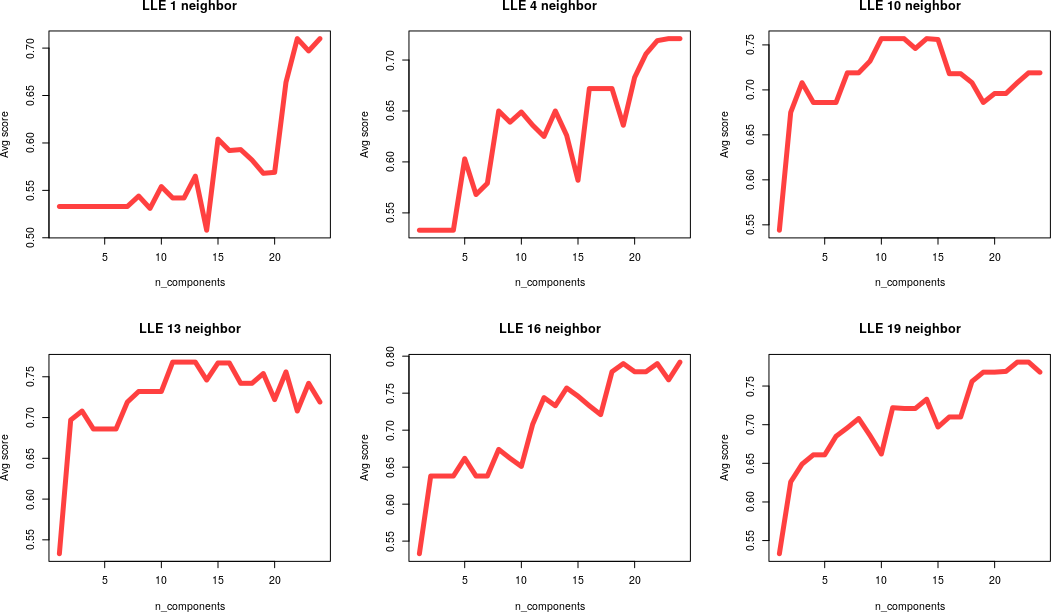
\includegraphics[width=1\textwidth]{img/LLEwl_plots.png}
		\caption{LLE performance.}
		\label{svmLLESP}
	\end{minipage}        
\end{figure}
For each table the minimum, average, maximum scores and standard deviation are obtained performing a 10-Way cross validation and the accuracy scores noted with the symbol $*$ are the best ones.
From Table \ref{table:svmPPI} we can see that, considering the shortest path kernel, the best scores are provided by the delta kernel, that as we have seen it keeps information about the number of nodes in the graphs and number of shortest path per weight. The results obtained by the SVM without manifold learning give us the idea that the WL kernel tends to better describe the similarity between the graphs in the manifold, since we can see that in general the best maximum results are obtained from it. An interesting observation on WL kernel is that we can see that increasing the depth $h$ (number of iterations) the scores do not improve, meaning that the kernel tries to consider new subtrees, reducing the locality information, that are not useful.\\
Table \ref{table:svmPPISPML} is obtained considering the shortest path kernel and the two manifold learning techniques, then different results are proposed in order to better understand how the results change with different numbers of neighbors and dimensions. Combining the results obtained from Table \ref{table:svmPPISPML}, Figure \ref{svmIsoSP} and Figure \ref{svmLLESP} we can see that the best results are obtained increasing the number of components, that result is given by the fact that we are giving more degrees of freedom to the embedding algorithms. The choice of the number of neighbors seems to be strongly dependent on the number of components, since when we increase the number of neighbors the best results are provided with an high number of components. The unique difference is given by LLE, since we can see from  Figure \ref{svmLLESP} that when we increase the number of neighbors, having too high number of components seems to be not efficient and we have a decrease on the accuracy scores. Considering instead the comparison between the two manifold techniques Isomap seems to produce relative better results respect to LLE.\\
Table \ref{table:svmPPIWLML}, Figure \ref{svmIsoSP} and Figure \ref{svmLLESP} are obtained considering the WL kernel with depth equals to 2 ($h= 2$). Here we can see some differences respect to the previous analysis. Isomap provides again the best scores, but now when the number of neighbors increases the better results are provided when the number of components remains restricted and does not increase to much, otherwise we can see a negative trend of the scores. LLE instead works very well when we increase the number of components and with high number of neighbors. From a certain point of view with LLE the most significant parameter here seems to be the number of neighbors that the algorithm use.

\subsection{Shock dataset}
In this section are proposed the scores obtained considering the shock dataset, which consists on graphs representing 2D shapes. The particularity of this dataset is that it is composed not just by $2$ classes, like the previous one, but it contains $10$ different ones. In this case the classifier can apply two different strategies:
\begin{itemize}
	\item \textbf{one vs all}
	\item \textbf{one vs one}
\end{itemize}

The difference between the two strategies is the number of classifiers that it is necessary to learn, which strongly correlates with the decision boundary they create. Considering a dataset composed by $N$ different classes with the \textbf{One vs all} classifier will train one classifier per class, so that at the end we have $N$ classifiers. For class $i$ it will assume $i$-labels as positive and the rest as negative. In \textbf{One vs one} it will learn a separate classifier for each different pair of labels, leading to $\frac{N(N-1)}{2}$ classifiers.

The problem of the first solution is that it is sensible to possible imbalanced datasets, but efficient from a computational point of view. The One vs one instead has a greater complexity but deals better with imbalanced datasets.
\renewcommand{\arraystretch}{1.5}
\begin{table}[H]
	\centering
	\begin{tabularx}{\linewidth}{|Y|l|l|l|l|}
		\cline{1-5}
		\centering{\textbf{Kernel}} & \thead{min score} & \thead{avg score} & \thead{max score} & \thead{stand dev}\\
		
		\cline{1-5}
		\centering \textit{SP kernel - step} & $0.35$ & $0.455$ & $0.65$ & $0.11$\\
		\cline{1-5}
		
		\cline{1-5}
		\centering \textit{SP kernel - delta} & $0.3$ & $0.425$ & $0.65$ & $0.129$\\
		\cline{1-5}
		
		\cline{1-5}
		\centering \textit{$WL_1$ kernel} & $0.25$ & $0.415$ & $0.6$ & $0.15$\\
		\cline{1-5}
		
		\cline{1-5}
		\centering \textit{$WL_2$ kernel} & $0.3$ & $0.41$ & $0.6$ & $0.15$\\
		\cline{1-5}
		
		\cline{1-5}
		\centering \textit{$WL_3$ kernel} & $0.35$ & $\mathbf{0.459^*}$ & $0.7$ & $0.117$\\
		\cline{1-5}
		
	\end{tabularx}
		\caption{Shock classification accuracy and std without m.l.}
		\label{table:svmShock}
\end{table}
\renewcommand{\arraystretch}{1}



\renewcommand{\arraystretch}{1.5}
\begin{table}[H]
	\centering
	\begin{tabular}{cc|c|c|c|c|l}
		\cline{3-6}
		& & \multicolumn{2}{ c| }{\textbf{Isomap}}& \multicolumn{2}{ c| }{\textbf{LLE}} \\ 
		\cline{1-6}
		\multicolumn{1}{ |c|  }{\#\textit{neighbors}}& \#\textit{dimensions}&\textit{avg} &\textit{std} & \textit{avg} & \textit{std} \\ 
		\cline{1-6}
		\multicolumn{1}{|c|}{4} & $1$ & $0.265$ & $0.092$ & $0.19$ & $0.086$\\
		\cline{1-6}
		\multicolumn{1}{|c|}{4}& $6$ & $0.435$ & $0.087$ & $0.27$ & $0.051$\\
		\cline{1-6}
		\multicolumn{1}{|c|}{10} & $6$ & $0.36$ & $0.099$ & $0.44$ & $0.087$\\
		\cline{1-6}
		\multicolumn{1}{|c|}{10} & $18$ & $0.35$ & $0.155$ & $0.375$ & $0.163$\\
		\cline{1-6}
		\multicolumn{1}{|c|}{13} & $2$ & $0.315$ & $0.084$ & $0.23$ & $0.075$\\
		\cline{1-6}
		\multicolumn{1}{|c|}{13} & $5$ & $\mathbf{0.44^*}$ & $\mathbf{0.1^*}$ & $0.44$ & $0.089$\\
		\cline{1-6}
		\multicolumn{1}{|c|}{13} & $13$ & $0.4$ & $0.147$ & $0.4$ & $0.128$\\
		\cline{1-6}
		\multicolumn{1}{|c|}{16} & $6$ & $0.35$ & $0.105$ & $0.4$ & $0.089$\\
		\cline{1-6}
		
		\multicolumn{1}{|c|}{16} & $16$ & $0.395$ & $0.117$ & $0.45$ & $0.13$\\
		\cline{1-6}
		
		\multicolumn{1}{|c|}{19} & $11$ & $0.4$ & $0.112$ & $0.38$ & $0.117$\\
		\cline{1-6}
		\multicolumn{1}{|c|}{19} & $17$ & $0.385$ & $0.129$ & $\mathbf{0.46^*}$ & $\mathbf{0.122^*}$\\
		\cline{1-6}
	\end{tabular}
		\caption{Shock classification accuracy and std with m.l. and shortest path kernel.}
		\label{table:shockMLSP}
\end{table}
\renewcommand{\arraystretch}{1}

\begin{figure}[H]
	\begin{minipage}[t]{0.5\linewidth}
		\centering
		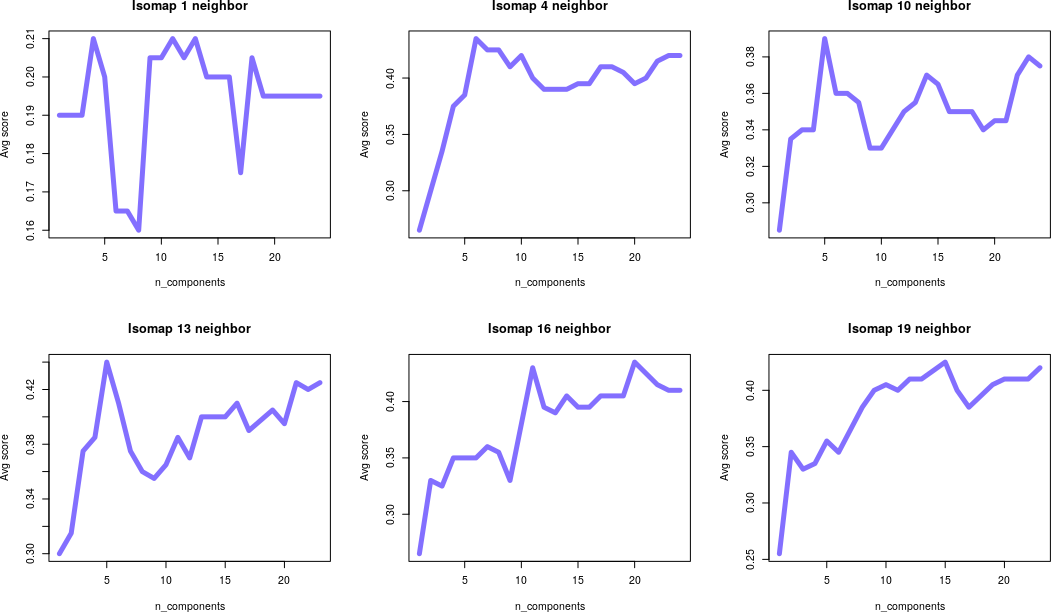
\includegraphics[width=1\textwidth]{img/isomapsp_shock.png}
		\caption{Isomap performance.}
		\label{shockSPISO}
	\end{minipage}
	\hspace{0.1cm}
	\begin{minipage}[t]{0.5\linewidth} 
		\centering
		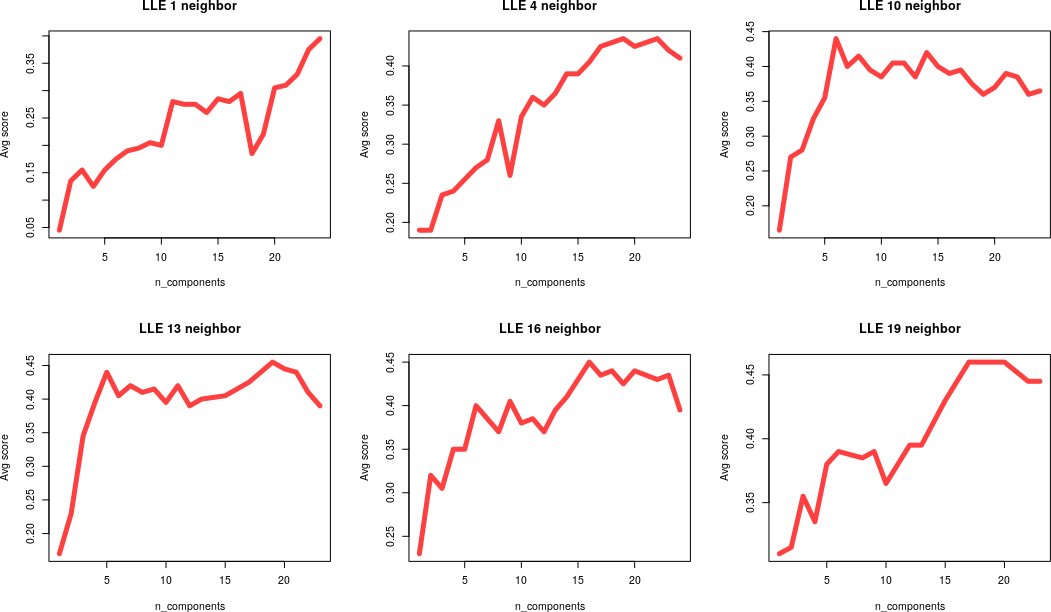
\includegraphics[width=1\textwidth]{img/LLEsp_shock.png}
		\caption{LLE performance.}
		\label{shockSPLLE}
	\end{minipage}        
\end{figure}

In table \ref{table:svmShock} we can see that the performance applying any kind of graph kernel and then a linear SVM the scores are not good. This means that the dataset is not simple and probably using a linear classifier is not the right way to proceed and more complex techniques should be adopted. In our case we just want to evaluate the performance of applying or not a manifold learning technique independently on the type of SVM. The results suggest that the Weisfeiler-Lehman kernel produces better results increasing the depth $h$ used by the algorithm, meaning that the considering more information coming from other subtrees of the shapes can be useful for classification and mitigate different shapes.\\
Table \ref{table:shockMLSP}, which is obtained considering the shortest path kernel and the two manifold learning techniques, shows better results in terms of average score, meaning that Isomap and LLE improve class separability over the manifold. Regarding the parameters, Figure \ref{shockSPISO} and Figure \ref{shockSPLLE} suggest that it is better to pick large number of components and neighbors, giving more degrees of freedom. Comparing the two results, what we can see is that in general LLE works better than Isomap, enhancing the class separability.
\renewcommand{\arraystretch}{1.5}
\begin{table}[H]
	\centering
	\begin{tabular}{cc|c|c|c|c|l}
		\cline{3-6}
		& & \multicolumn{2}{ c| }{\textbf{Isomap}}& \multicolumn{2}{ c| }{\textbf{LLE}} \\ 
		\cline{1-6}
		\multicolumn{1}{ |c|  }{\#\textit{neighbors}}& \#\textit{dimensions}&\textit{avg} &\textit{std} & \textit{avg} & \textit{std} \\ 
				\cline{1-6}
		\multicolumn{1}{|c|}{4 } & $1$ & $0.14$ & $0.044$ & $0.155$ & $0.079$\\
		\cline{1-6}
		\multicolumn{1}{|c|}{4 }& $13$ & $0.38$ & $0.1$ & $0.4$ & $0.097$\\
		\cline{1-6}
		\multicolumn{1}{|c|}{4 }& $17$ & $0.38$ & $0.078$ & $0.465$ & $0.103$\\
		\cline{1-6}
		\multicolumn{1}{|c|}{10} & $6$ & $0.375$ & $0.115$ & $0.215$ & $0.063$\\
		\cline{1-6}
		\multicolumn{1}{|c|}{10} & $18$ & $0.365$ & $0.132$ & $0.38$ & $0.119$\\
		\cline{1-6}
		\multicolumn{1}{|c|}{13} & $8$ & $0.345$ & $0.162$ & $0.295$ & $0.151$\\
		\cline{1-6}
		\multicolumn{1}{|c|}{13} & $15$ & $0.33$ & $0.15$ & $0.385$ & $0.123$\\
		\cline{1-6}
		\multicolumn{1}{|c|}{13} & $21$ & $0.39$ & $0.109$ & $0.39$ & $0.139$\\
		\cline{1-6}
		\multicolumn{1}{|c|}{16} & $10$ & $0.41$ & $0.136$ & $0.455$ & $0.079$\\
		\cline{1-6}
		\multicolumn{1}{|c|}{19} & $10$ & $0.37$ & $0.114$ & $\mathbf{0.485^*}$ & $\mathbf{0.063^*}$\\
		\cline{1-6}
		\multicolumn{1}{|c|}{21} & $6$ & $0.395$ & $0.14$ & $0.315$ & $0.078$\\
		\cline{1-6}
		\multicolumn{1}{|c|}{21} & $12$ & $0.37$ & $0.114$ & $0.465$ & $0.059$\\
		\cline{1-6}
		\multicolumn{1}{|c|}{26} & $9$ & $0.425$ & $0.145$ & $0.36$ & $0.077$\\
		\cline{1-6}
		\multicolumn{1}{|c|}{26} & $19$ & $\mathbf{0.465^*}$ & $\mathbf{0.116^*}$ & $0.435$ & $0.095$\\
		\cline{1-6}
	\end{tabular}
		\caption{Shock classification accuracy and std with m.l. and Weisfeiler-Lehman kernel.}
		\label{table:svmWLML}
\end{table}
\renewcommand{\arraystretch}{1}


\begin{figure}[H]
	\begin{minipage}[t]{0.5\linewidth}
		\centering
		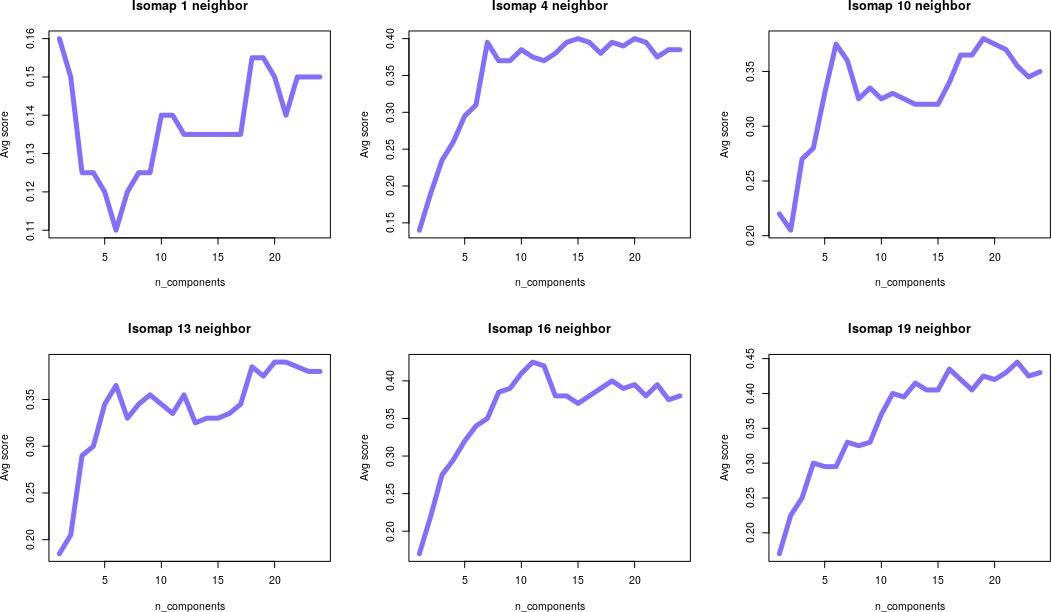
\includegraphics[width=1\textwidth]{img/IsomapWL_shock.png}
		\caption{Isomap performance.}
		\label{isoWLML}
	\end{minipage}
	\hspace{0.1cm}
	\begin{minipage}[t]{0.5\linewidth} 
		\centering
		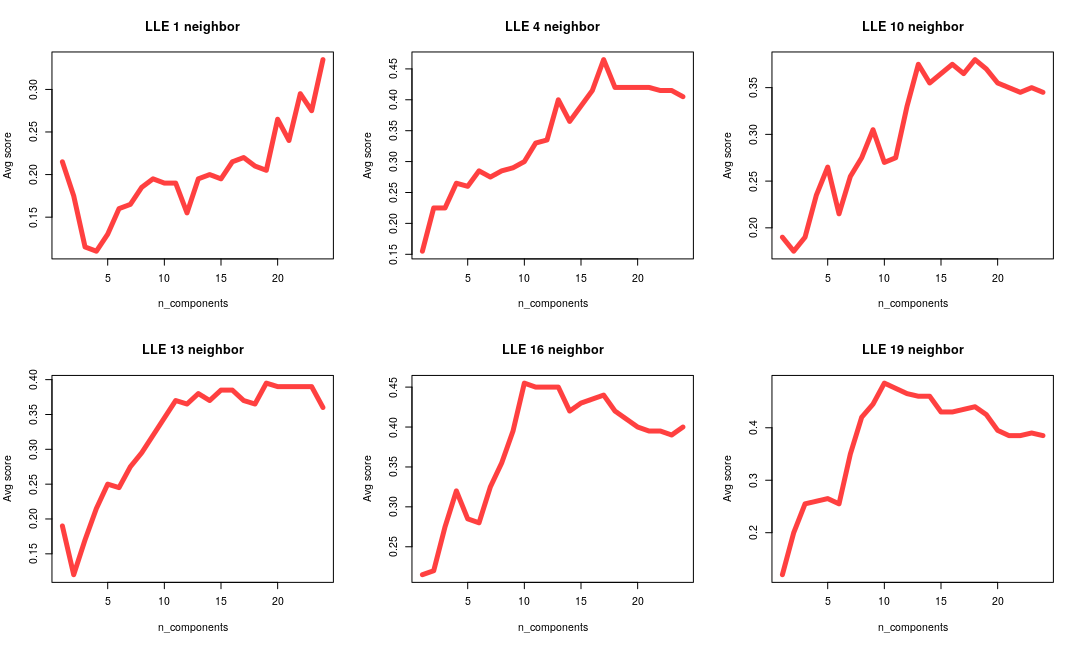
\includegraphics[width=1\textwidth]{img/LLEwl_shock.png}
		\caption{LLE performance.}
		\label{lleWLML}
	\end{minipage}        
\end{figure}
Considering table \ref{table:svmWLML} we can see that the effect of manifold learning seems gives  a slight enhancing on the class separability. It is also possible to observe that the major improvement is given by LLE, instead Isomap starts to give better results when we increase a lot the number of dimensions and neighbors. Figure \ref{isoWLML} and Figure \ref{lleWLML} present the same pattern that we have previously analyzed, that is the manifold learning technique works well with a discrete number of degree of freedom and a tolerant number of neighbors.

\newpage

\section{Conclusion}
In this document, we have faced the problem of converting directly graph structures into exact vectorial form with the purpose of using the classical machine learning techniques over them. We have seen that there is not a precise definition useful to convert a graph into a vector, but it is possible to stem the problem taking advantage on the kernel trick strategy, which basically consists on computing the similarity between the given graphs in a proper space. We have seen  graph kernels that can be applied and each of them considers different types of information (labels, topology, etc.). In particular we have analyzed the theoretical aspects, properties and complexities of two well known graph kernels, Shortest-Path and Weisfeiler-Lehman kernel. \\
Another aspect of this assignment was to give also some theoretical knowledges and properties about manifold learning algorithms, commonly useful for dimensionality reduction. Two important manifold learning algorithms, Isomap and Local Linear Embedding, were analyzed. The main goal was to evaluate if the two algorithms could enhance the classes separability projecting the original manifold in a low-dimensional embedding. Then, in order to give a correct and unbiased analysis, the followed strategy have proposed different linear SVM classifiers, based or not on the application of a manifold techniques, learned over two datasets of graphs (PPI and Shock).
Analyzing the obtained results with the two datasets, we have seen that the application of both the manifold learning algorithms brought to a slight improvement of the obtained scores, meaning that they have enhanced the class separability a little bit. Of course another important aspect is that with any manifold learning technique we are embedding the original data-space into a new one which is composed by less components, meaning that it is possible to reduce the computational cost time and space required to analyze and store data. \\
Manifold learning techniques so can be useful to reduce data with a non-linear dimensionality reduction strategies and this also improving the accuracy scores, obtained from a general classifier. It is important to notice that the proposed manifold learning techniques work considering two fundamental hyper-parameters, number of neighbors and number of components. During the analysis step we have also seen that the choice of the two in fundamental, since a small number of components could not give enough degrees of freedom and the number of neighbors decide how many local information should be considered.\\
More in general, we have observed that in most of the cases the separation of the data could be increased after applying manifold learning on the original kernels by picking the right hyper-parameters. 
\end{document}
